\documentclass[12pt]{report}
\usepackage{lipsum}
\usepackage{mathtools}
\usepackage{array}
\usepackage{colortbl}
\usepackage{chemfig}
\usepackage{csvsimple}
\RequirePackage[left=3cm,top=1.5cm,right=3cm,bottom=2.5cm,nohead]{geometry}
\usepackage{sectsty}

\sectionfont{\fontsize{17}{15}\selectfont}

\begin{document}

\begin{titlepage}
	\begin{center}
		\vspace*{1cm}
		
		{\Huge \textbf{Social distancing detection with computer vision techniques}}
		
		\vspace{0.5cm}
	
		
		\vspace{1.5cm}
		
		\textbf{Lee Hoang}
		
		\vfill
		
		\vspace{0.8cm}
		
		BSc Computer Science\\
		City University, London\\
		Date
		
	\end{center}
\end{titlepage}

\tableofcontents

\chapter{Introduction}

\chapter{Output Summary}

\chapter{Background Research}
\section{What is computer vision?}

Computer vision (CV) is a scientific discipline that studies how computer scan efficiently perceive, process, and understand information from visual data such as images and videos.

\vspace{2mm}

As humans, we can classify three-dimensional objects with ease, whether the pictures are the same object with different colours or angles, we are good at determining the object we are classifying. 
Computer vision has been developed to detect edges from a pixelated image, face detection, and has been used to develop 3D models from a snapshot yet the technology we have today could be compared to a young child's biological vision. 

\vspace{2mm}

Computer vision is used in various real world application such as traffic surveillance or medical imaging (SZELISKI, 2020), where people are now able to utilize magnetic resonance imaging (MRI) to safely analysis the heart wall motion where the end result is a 3d model of the heart pumping (Metaxas, 1997). 

\vspace{2mm}

In recent years, computer vision has been adapting deep learning algorithms to efficiently classify unseen objects within pixel images and videos. 


\section{Deep learning}

Deep learning uses artificial intelligence (AI) to try and simulate the choices that a human brain will make. Problems that have regression or classification outputs can be solved by passing data/inputs through artificial neurons which were previously tweaked for the specific problem by training data. There are many different variants of deep learning algorithms such as Artificial Neural Networks (ANN) or Long Short-Term Memory (LSTM) Networks (Hochreiter, 1997) which build onto each other.

\subsection{Neural networks (NN)}

Neural networks is a network formed of interconnected perceptrons which each carry weights and biases. The weights (w) and biases (b) are each represented by a float value which are used to multiply and add to the input respectively. The outcome is then put into an activation function (e.g. ReLU or sigmoid) which determines if the neuron should be activated. These activations chain together to output a value of what the neural network thinks the solution is. 

\vspace{5 mm}

\begin{centering}
	
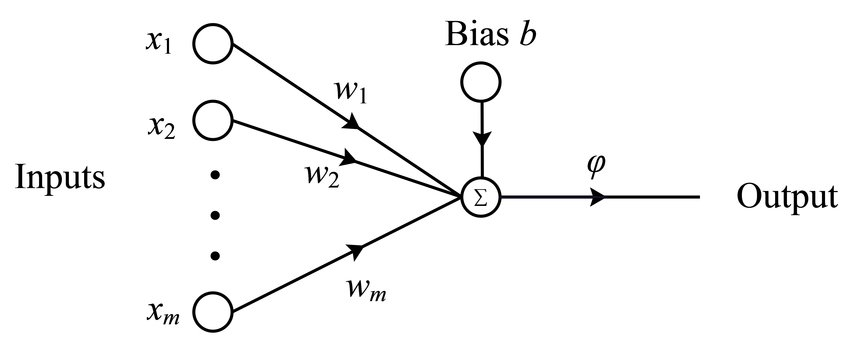
\includegraphics[width=100mm]{./images/weights and biases.png}

{Figure 1: A single perceptron with inputs, weights, and biases}

\end{centering}

\vspace{5 mm}

The values of weights and biases are updated when training data is pass through the network using back propagation, adjusting their values depending on the actual and network's solution to the problem. A network can have multiple layers of several perceptrons in order to solve more complex problems, but has the down side of overfitting the accuracy of the output.


\subsection{Convolutional neural networks (CNN)}

CNNs builds upon the NN, specialising in working with grid-structured data such as images or videos. Unlike NN which takes in a 1 dimensional vector as its input, CNN uses tensors (high dimensional vector/matrix) for processing images. The convolutional layer of the network includes kernels/filters (a type of matrix) which efficiently detects features within an image by calculate the sum of the kernel multiplied by a subgrid of the image. These filters are trained to extract details within the images, and to make better predictions over the course of training. Different techniques can be applied such padding to reduce the lost of data when filtering.

\vspace{2mm}

The information about the deep learning architectures have been discussed were influenced by taking part in the 'Introduction to AI' (IN3062) and 'Programming and Mathematics for Artificial Intelligence' (IN3063) module at City University.

\section{WILDTRACK dataset}

The 'WILDTRACK' dataset provides footage of pedestrians from 7 different angle, each video having a length of 35 minutes and were filmed using three 'GoPro Hero 4' and four 'GoPro Hero 3' at high resolution (1920x1080). The location of the video took place near a public research university called ETH Zurich, Switzerland. The cameras used were calibrated to allow for precise calculations when wanting the distance between two objects.

\vspace{2mm}

While there are other datasets that offer similar features such as the 'EPFL-RLC' dataset, the videos themselves do not contain the same density of pedestrians relative to the 'WILDTRACK' dataset.Footage from other datasets showcase people who are more static, making it less challenging for the project.

\subsection{Research papers with WILDTRACK dataset}

There are many published research papers that have used this dataset for their own project. For example, a research paper that was dedicated to detecting the same pedestrian using all camera footage and creating a shared top down view of the 'point of interest' which indicates the location of the pedestrians (López-Cifuentes A. 2018). What was interesting about this paper was that the author used another dataset that did not include calibrated cameras. When comparing the results at the end, the accuracy of the 'WILDTRACK' was marginally better as the other dataset had calibration errors, therefore the 'point of interest' were at different locations when looking at the shared top down view.


\section{Existing systems}

Many different social distancing detections have been made ever since the outbreak of the corona virus. Most of the systems use deep learning architectures paired with the OpenCV library to help classify pedestrians within a video.

\subsection{Example (Y. C. Hou, 2020)}

This system uses a combination of the YOLO (You Only Look Once) model with the COCO (Common Objects in Context) dataset to train their model. The goal of the project was to produce a top down view of the pedestrians, showing the distance between each person who were identified within the frame. The results of the system were very accurate, as they were able to make use of calibrated cameras. What was very interesting about the project is that some pedestrians were not classified due to hiding behind others. This showcases the limitation of the dataset used, as there were no overlapping footage of the field of view. Further improvements to the system were suggested such as mask and human body temperature detection. The system overall is similar to what this project will achieve with the difference of dataset.

\chapter{Method}

\section{Agile development}

An agile approach with sprints were used during the development of the project. The approach gave time to reflect and adjust the work being done through out the weeks while allowing focus on the core functionalities of the software being produced. 

The outcome of each sprint allowed for early prototypes of the system, easier analysis on code and product, and fixing any bugs within the code. The consequences of only partially completing a sprint's objective can be solved by adding more time for further development. Partially completion of the sprints are inevitable therefore spacing out the sprints instead of one immediately after the other will help allocate more time. 

\section{Management tools}

A diary is used to record sprints and work done throughout the week, recording the results produced and research done in order to produce code. Any images/video footage used in the dataset are copied and backed up into another folder for future reference. A simple Gantt chart is used to keep the work flow on track while also updating the chart to allocate time for sprints.

\subsection{Version control}

GitHub was used to store previous versions of the code used for the project. This is in case of any mistakes made during development, backup versions of the project can be restored. GitHub can allow the user to backup their version no matter how small the changes are, providing flexibility throughout the project. 


\section{Deep learning architectures for object detection}

Deep learning has been a foundation for modern computer vision, allowing object detection to be 'automatic' by training a CNN which tunes itself after each batch of training data, then being further developed by implementing algorithms for object detection which only requires one pass through the network. This project will specifically be using yolov3.

\subsection{YOLO (You Only Look Once)}

YOLO is a object detection architecture that uses convolutional neural networks to divide the image/input into a grid. Each box in the grid is then associated with a high dimensional vector which record data such as: if there is an object within the grid, the predicted position of the bounding box, and the class id of the object. The vector can be expanded if there is more than one object within the box which is called anchor boxes. See appendix 1 for a flowchart of YOLO.

\vspace{2mm}

It is possible for the architecture to identify the same object twice within the same box creating redundancy. Since the predictions are based on probability, the architecture chooses the highest probability and uses there bounding box to identify the object. This feature is called 'Non-Max suppression'.

\vspace{2mm}

There are many versions of the 'yolo' such as 'yolov2' but during 2018, 'yolov3' was released (REDMON J. 2018). When comparing to previous versions, it offers an increase in speed and efficiency when computing while also providing a better backbone classifier (The core convolutional neural network). 

\vspace{2mm}
There are also different models of 'yolov3' that perform better speed wise but at the cost of accuracy such as 'yolov3-tiny' which can compute videos at 220 frames per second (Benchmarked with 4 Titan X graphic cards). This project specifically will use 'yolov3-320' which will detect objects within a video at 45 frames per second while still having good accuracy. The reason for using this model is that realistically, cameras used in offices or public areas for surveillance will most likely be around 30 frames per second.

\vspace{2mm}

While this method of object detection is proven to be very effective, it comes with the drawback of not being very flexible when wanting to change the overall structure of the neural network. Its very likely that tweaking the structure if possible could make the outcome of the object detection worst, by also spoils the chances of improving it.

\section{Pre-trained models (With COCO dataset)}

The Microsoft 'COCO' (Common Objects in Context) dataset is a large-scale object detection dataset that contains over 330,000 images and more than 80 different object categories. This project used a pre-trained 'yolov3-320' model with the 'COCO' dataset to detect people within an image. The reasoning for using this is that the dataset is very large, and will take several days to train the network. In comparison, downloading the pre-trained weights (Redmon, 2021) took a few minutes. 

\vspace{2mm}

Another reason for using 'COCO' is that it is a well documented dataset (Lin et al., 2021), designed to help improve 'image classification' with images that contain multiple objects.

\vspace{2mm}

The objects that are in the dataset range from living beings such as 'person' and 'cat' to everyday objects such as 'bottle' and 'cup'. The main focus of the project is to detect 'person', therefore we will need to filter out the other objects within the code, but this means that the forward pass in the neural network will still detect other objects, possibly affecting the time spent to compute a simple image. 

\section{Hardware used}

The results were produced with a Intel Core i7-7700K and a Nvidia GeForce GTX 1080. The GPU is used to speed up the process of forwarding each frame of the video to the network. While speed is a factor in a real time software, this report mainly focuses on the detection of social distancing, therefore the results of the report can be replicated with a CPU only.
\section{Programming language and libraries}

This section discusses the chosen programming language and libraries used in the project, giving examples of functionalities within the coding aspect.

\subsection*{Python}

Python was chosen for flexibility when organising and presenting code through out the project. Python allows the user to call modules from different files that contained reusable classes and functions, making the overall structure of the code less cluttered.

\vspace{2mm}

Python has compatibility with libraries needed for the project which were installed using 'pip' which is a package management system.

\subsection*{NumPy}

NumPy specialises in matrix/array arithmetic, being able compute high dimensional matrix multiplication with ease. For this project, the project use NumPy for generating matrix transformations and to concatenate matrices to generate a side panel for the top down view. 

\subsection*{OpenCV}

OpenCV is a cross-platform library which can be used to develop real-time computer vision applications. OpenCV can be used to utilise the pre-trained weights previously discussed, allowing to input an image and filter out the objects within the image.

\vspace{2mm}

Another functionality of the OpenCV library is image transformation, transforming a plane in an image to a 'flat surface'.


\subsection*{Matplotlib with Seaborn}

Matplotlib is a library that specialises in creating plots and graphs. The seaborn library will be primarily used for the presentation of the plots from matplotlib.

\section{Dataset preparation}

The dataset features 7 videos of pedestrians walking in a public space (each video are at different angles) that are each 35 minutes long and are shot at 60 frames per second. It also includes image subsets of the videos, each one taken every tenth of a second from the video with a resolution of 1920x1080. These images are already post-processed to remove distortion.

\vspace{2mm}

Due to the large dataset, this project will be utilising samples of screenshots from each camera used to test the capabilities of the 'yolov3' architecture, and will be augmented with artificial noise which allows for extreme test.

\vspace{2mm}

The videos are sampled to 5 - 10 second clips using windows video editor. Each clip will contain a variety of pedestrians doing different actions such as being stationary or walking side by side in a group. The clips are still at 1920x1080 resolution, but are reduced to 30 frames per second. This is because the industry standard for surveillance cameras are 30 frames per second and it will take less time to compute a video.

\vspace{2mm}

Figure 4.1 is a table that labels each image/video used in the report, giving a name that will be referenced throughout the report, what camera the video came from, the time the clip started from the original video and length or the frame it came from, and a short description on the main activity in the image/clip.

\vspace{5mm}

\begin{center}
\footnotesize
	\begin{tabular}{|p{2.2cm}|l|p{1.8cm}|p{2cm}|p{5cm}|}
		\hline
		Image/video name & Camera & Start time /frame & Length (Seconds) & Description \\
		\hline
		image 1 & 1 & 0 & N/A & A Large crowd in the background with a group of 3 in the middle. \\
		\hline
		image 2 & 4 & 730 & N/A & A person blocking the camera view of another person. \\
		\hline
		image 3 & 4 & 950 & N/A & A cluster of people close to the camera and in the background. \\
		\hline
		image 4 & 5 & 30 & N/A & Two people standing next to each other with back facing the camera. \\
		\hline
		video 1 & 1 & 15:02 & 8 & Group of stationary people with a person walking by. \\
		\hline
		video 2 & 1 & 19:54 & 8 & A single person walking past. \\
		\hline
		video 3 & 2 & 23:27 & 6 & Two people walking past each other with close proximity. \\
		\hline
		video 4 & 2 & 16:43 & 10 & Group of four people walking side by side. \\
		\hline
		video 5 & 3 & 1:00 & 10 & Large crowd of people walking past. \\
		\hline
		video 6 & 3 & 32:49 & 7 & Two people making contact with each other. \\ 
		\hline
		video 7 & 6 & 7:05 & 8 & Two people walking together with their backs to the camera. \\
		\hline
		video 8 & 6 & 22:33 & 8 & A cluster of four people walking with their backs to the camera. \\
		\hline 
		video 9 & 7 & 29:05 & 8 & Two people hugging each other. \\
		\hline
		video 10 & 7 & 14:30 & 8 & Stationary group and a moving group side by side. \\
		\hline
	\end{tabular}
\vspace{4mm}

{Figure 4.1: Table of images and video samples used.}

\end{center}

\section{System model}

This section discusses the overall flow of the system, how it uses pre-trained model, and the different approaches to detecting close proximity 

\vspace{2mm}

The flow of the system was model with a activity diagram (figure 4.2), showcasing the step by step process of the overall system and how it interacts with 'yolov3'. The system has three different methods to calculate close proximity of two people and will be later discussed in the results section.

\vspace{2mm}

The goal of the system is to mark pedestrians who are close to each other with a red bounding box and the people who are not close with a green bounding box. The system should be able to mark these onto a side panel which represents the top down view of the image. If the input is a video, then the system should calculate all of the step for every frame within the video, the outcome should be the same video but with new annotations included.
 
\vspace{10mm}

\begin{centering}
	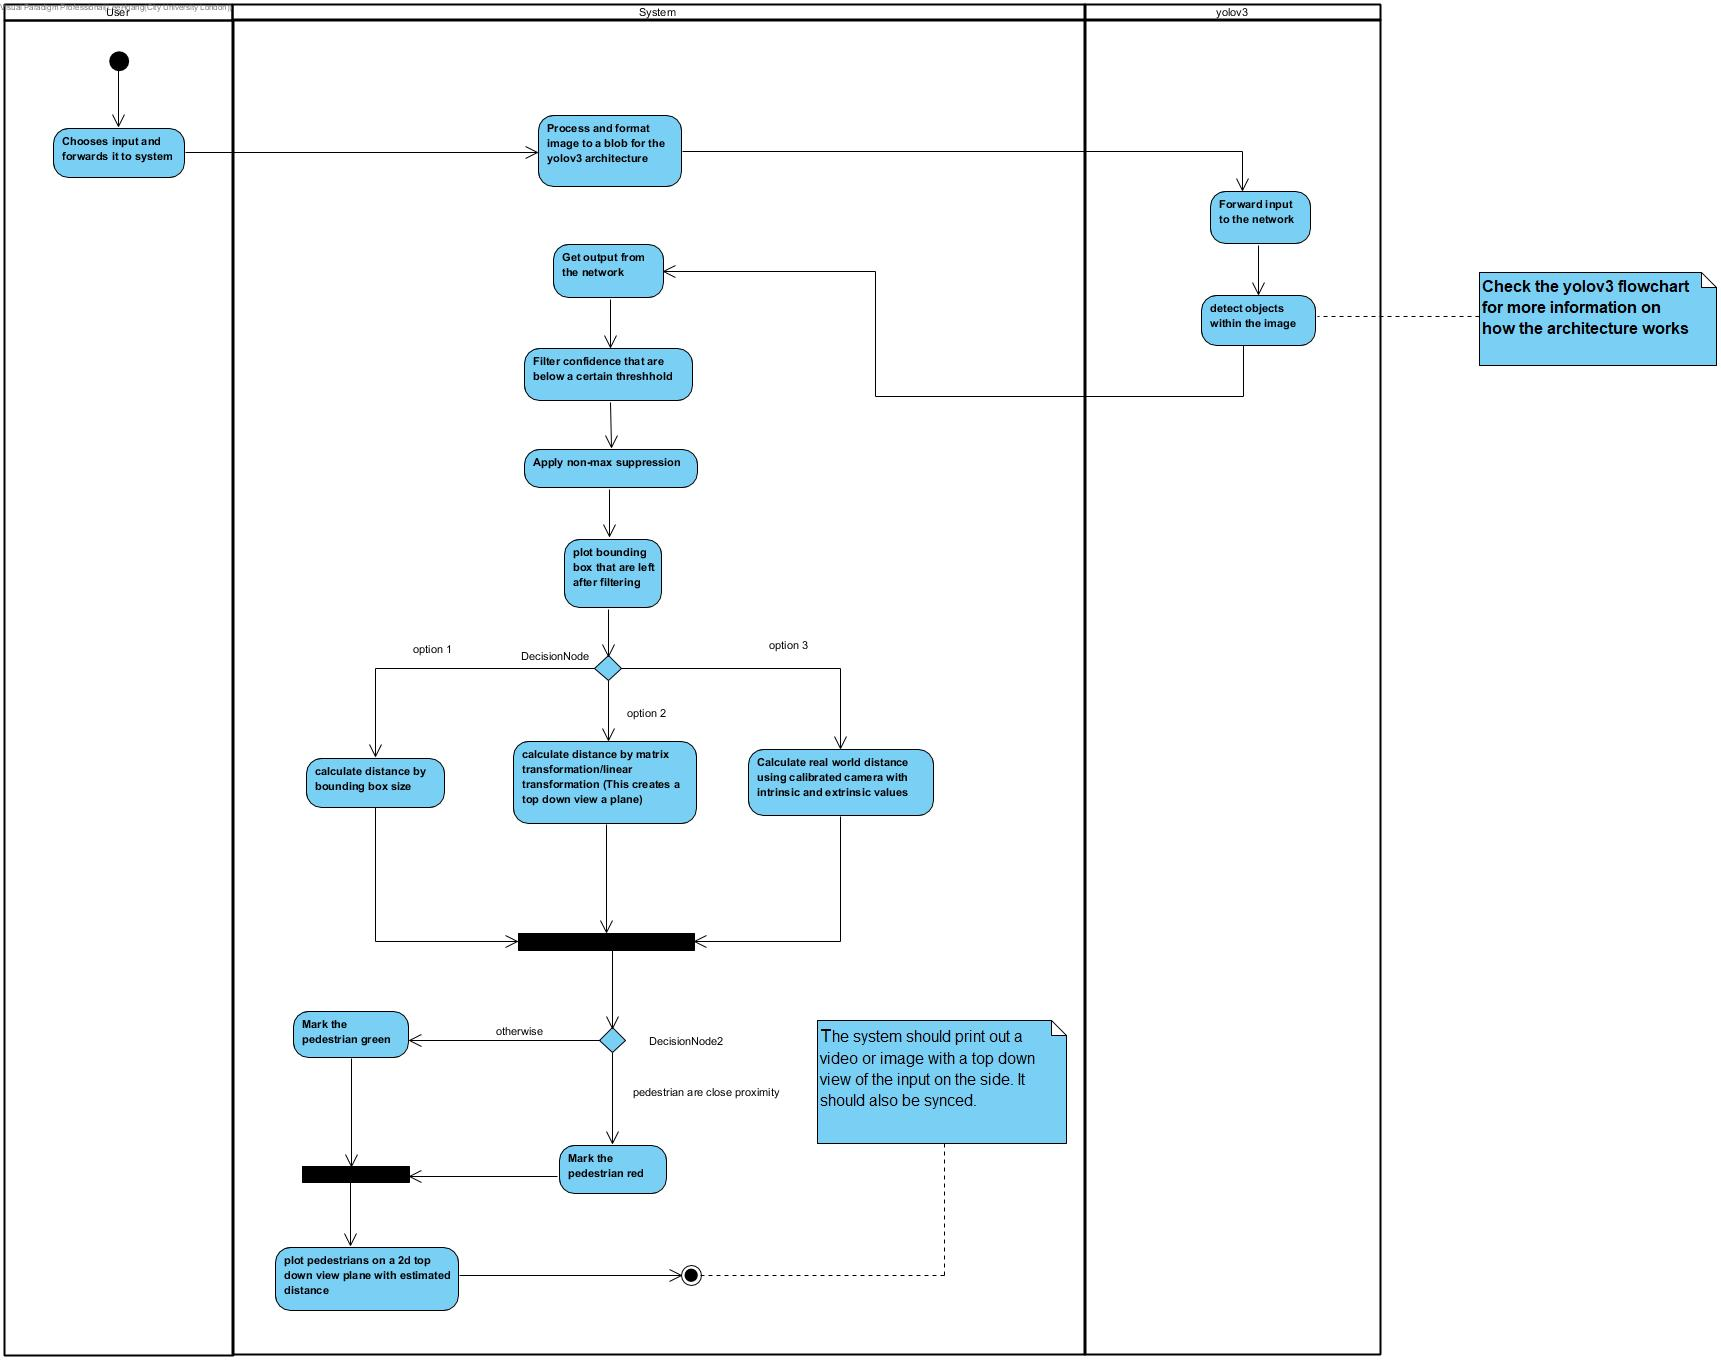
\includegraphics[width=170mm]{./images/system design.jpg}
	{Figure 4.2: Activity diagram describing the system pipeline}
	
\end{centering}

\vspace{10mm}

A class diagram (appendix 2) was created to show the functions that occur through out the system with the inputs and outputs. Each function also includes the key parameters needed, as well as the function data type.

\section{Development phases}

The project has several development phases to give time to thoroughly test each feature of the system. These phases will be done in chronological order and will each be treated as a sprint.

\subsection*{Object detection with YOLO}

This phase will focus on forwarding images to the network to test how well the object detection works. The images used in the testing will have different density of population in the image, where some images will contain people overlapping another. The same images will also be artificially augmented by adding noise or rotation to image to limit test the architecture. This phase will also be testing videos as inputs, the main measurement of success will be how smooth each individual is tracked through out the processing.

\subsection*{Detecting social distancing by bounding box distance}

By using the found bounding box in the first phase, the program should be able to compute the distance between two people using pixels as a estimated measurement. This will be tested with different camera angles to see how effective the implementation is.

\subsection*{Detecting social distancing by matrix transformation}

This method can be achieved by using the OpenCV library to calculate a matrix that transforms a quadrilateral in an image that is marked with 4 points to a square/rectangle image. this transformation is a combination of rotation, translation and shears. This will be tested with videos before and after distortion.

\subsection*{Detecting social distancing by camera calibration}

The dataset provides intrinsic and extrinsic values for the cameras used. This enables the project to convert pixel values to real world measurements, acquiring a very accurate solution to the problem. Using this method sucessfully will showcase how effective the other methods in comparison to each other.

\subsection*{Plotting pedestrians on a top down view of the image}

The system will create a side panel showcasing the topdown view of the pedestrians and if they are close to each other with a green or red highlight. This can be used to compared the social distancing detection methods.

\subsection*{Identifying groups of people and marking them 'safe'}


\chapter{Results}

This section discusses the results found throughout the project.

\section{Detecting objects with 'yolov3' (Analysis)}

OpenCV enabled the use of 'yolov3' with the built in functions of loading the weights of the neural network and forwarding an image to output the objects detected. 

\vspace{2mm}

The first image that was forwarded was 'image 2' (figure 5.1). The main focus of using this specific image was to look at how well the model detected people who were overlapping each other. The outcome of model was over 5,000 objects detected within the image, taking 0.54 seconds to compute. The amount of objects detected might seem unnecessary, but the model was trained to detect 80 different objects, therefore will provide a large number of classifications per image.

\vspace{2mm}

Each bounding box that the model outputs comes with a probability that the object detected is the correct classification. Therefore objects that are a 'person' could also have a probability of being identified as a 'car'.

\subsection{Filtering classification methods}

The probabilities can be filtered by extracting the highest probability that the model gave to a object within the image by using the argmax function that NumPy provides. This method of filtering removes 98.75 percent of the objects identified by YOLO, as it chooses 1 object from 80 different classifications, reducing the total number of objects left to 71 for 'image 2'.

\vspace{2mm}

Another method of filtering was to apply a probability threshold. Increasing the threshold filtrates all probabilities that are below a certain percentage. Figure 5.1 shows a plot that focuses on the amount of objects that are detected with different levels of confidence with a 2 percent increment. Having a really high percentage means that model almost guarantees the object classification if correct. This has the draw back of not being able to detect any pedestrians far in the background (Appendix 3a), as they have lower classification percentage that the people closer to the camera. It is more optimal to have a lower percentage in 'image 2' as the system is able to pick up people who are hiding behind others even though they are close to the front of the camera which is important in an office environment.

\begin{center}
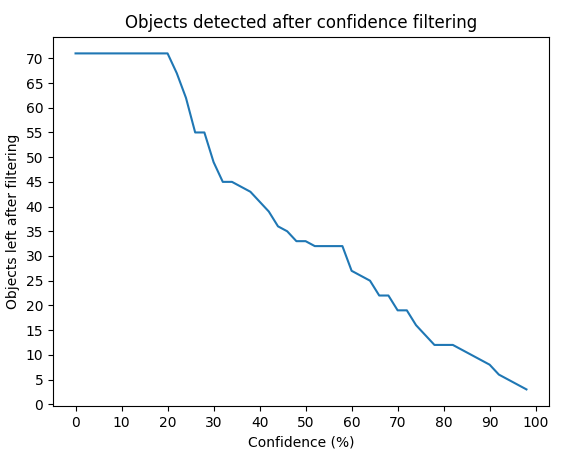
\includegraphics[width=75mm]{./images/appendix/ConfidencePlot.PNG}
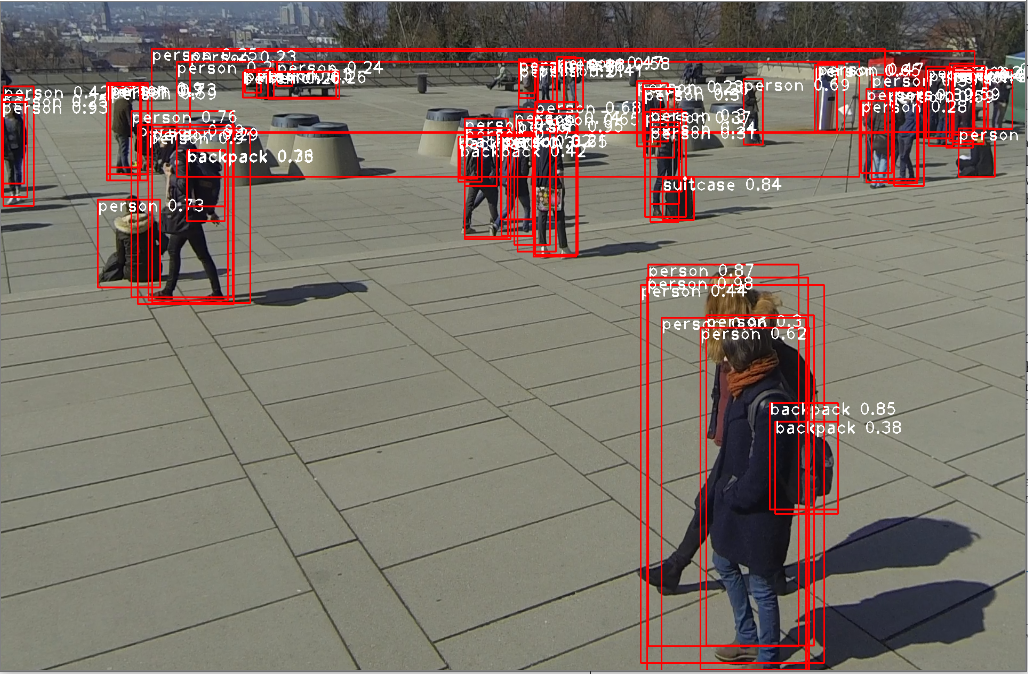
\includegraphics[width=75mm]{./images/zeroConfidence.PNG}

\vspace{3mm}
{\footnotesize Figure 5.1: Confidence plot on 'image 2' (left) and 'image 2' with 0 percent confidence (right)}
\end{center}

\subsection*{Non-max suppression}

The choice of having a small confidence has a clear down side of an increased amount of overlapping bounding boxes on the same object (Figure 5.1). To reduce the overlaps, the system uses non-max suppression which was discussed in the method section.  

\vspace{2mm}

Non-max suppression (NMS) has a parameter that can be tuned to either increase or decrease the effectiveness of NMS where a smaller parameter filters more bounding boxes on the same object. The function was testing with 'image 2' (30 percent confidence). Opposite to the confidence parameter, having an extremely low parameter for NMS loses too much information in the process. 

\vspace{2mm}

In this image specifically using 0.1 as the parameter, the person who is hiding behind the other in front of the camera view is not being detected in the finished output and some people in the background also lost their bounding boxes. Losing the people in the background is less problematic if the system were to be used in an small office space, but, having a low parameter could harm the people who are hiding behind others as they will not be considered when calculating the social distancing. In this image, the person in front would be marked as 'safe' when calculating social distancing.

\vspace{2mm}

On the other hand, having a larger parameter value will keep too much information as there will be still be overlapping bounding boxes on the same object, not making full use of NMS. The reason why overlapping bounding boxes are bad for the final output of object detection is that when calculating if the person is social distancing, they will be seen as 'unsafe' even if there is no visible person next to them as the system relies on the position of the bounding boxes when calculating distance.

\vspace{2mm}

While there is a parameter value that voids all overlapping boxes and detects the person hiding behind the other in 'image 2' (value 0.6), the bounding box that NMS chose was suboptimal and was bigger than the person's body (Appendix 3b). Solving the problem by adjusting the 'yolov3' architecture can be difficult as the image itself was intentionally used as an extreme example and may even take humans a second to see that there is a person behind the other as there is only hair and a leg showing.

\vspace{2mm}

A higher camera angle when taking this picture could be a solution for hidden people, allowing for more exposure on the person's figure. Likely, a perfect angle for detecting people with this architecture would be close to a top down view of the floor which acts as a planar surface, allowing to see every single person in view without the worry of hiding behind someone else. Achieving a fully working object detection on the image goes beyond what is capable of the YOLO architecture. Moving forward, any frames within a video that experiences the same level of object interference will be seen as an 'outlier' frame for simplicity. 

\subsection{Image augmentation}

The purpose of testing object detection with images that are augmented is that the inputs we are working with are high quality 1080p images and videos. It is possible that the user who wants to use the finished product have cameras that do not match the quality of the ones shown throughout the results.

\vspace{2mm}

This test will use 'image 4' for a baseline example and will be augmented, mainly focusing on the two people who are next to each other on the left (Figure 5.2). The image was reduced to 1280x720 resolution. All variations of the image was processed with a confidence percentage of 50 and 0.5 for the NMS parameter. 

\vspace{2mm}

The images will have artificial noise added using a technique called 'salt and pepper' (adding black and white pixels to random spots). The amount of 'salt and pepper' that are added to an image can be controlled by a parameter that determines the probability that a pixel in the image will either turn black/white or stay the same where turning black and white are same probability. This technique is done manually using a 'for' loop where the loop goes through every pixel of the image. A number is rolled each time within the for loop and is not set, this means that running the program again with the same parameters may lead to different results.

\vspace{2mm}

The first test using 10 percent probability produced similar bounding boxes to the original image, with a slight difference of bounding box height/width and the probability of correct classification also varies. While it is only a sample of one, 'yolov3' seems to work well with different resolutions and noise as shown in figure 5.2, successfully identifying the two people who are on the left.

\vspace{2mm}

When increasing the intensity of noise, the bounding boxes that are shown decreases in quantity as the model is having a harder time determining the probability that the object is a 'person'. Augmenting the image to 50 percent noise (figure 5.2) made it so the object detector could not identify a 'person' with above 50 percent confidence. 

\vspace{2mm}

With a 0 percent confidence and without NMS (Appendix 3c), all variations of the images do identify the two people. This concludes that not having a high quality image may affect the probability that the system correctly classifies an object, but can be solved by lowering the confidence threshold. The drawback of having a lower quality camera is that it reduces the total amount of bounding boxes which may lead to people being unidentified by the system.


\begin{center}
	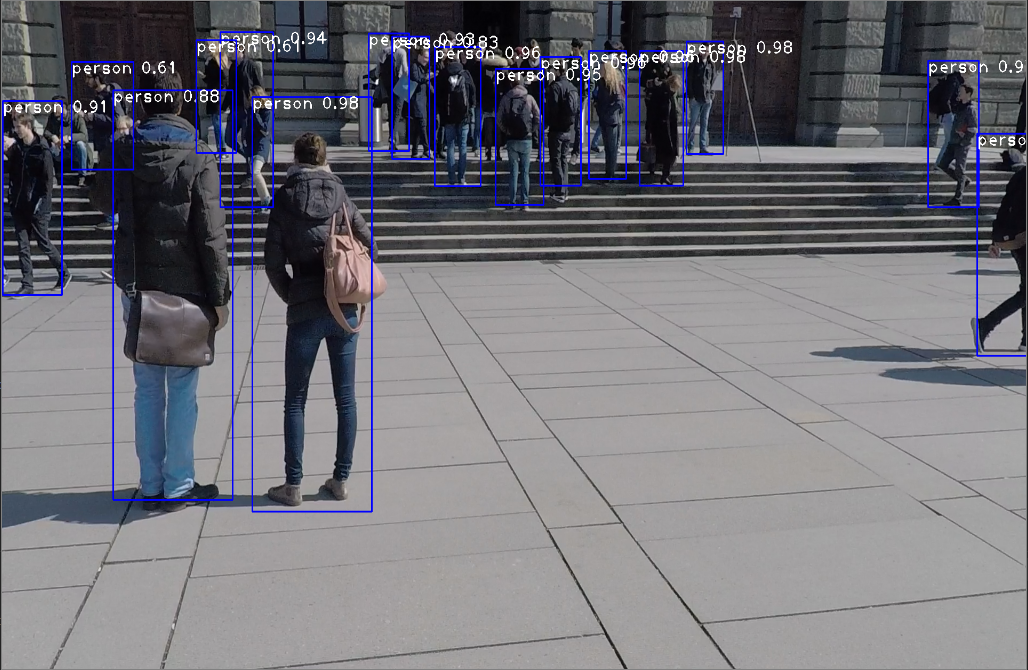
\includegraphics[width=65mm]{./images/image45050.PNG}
	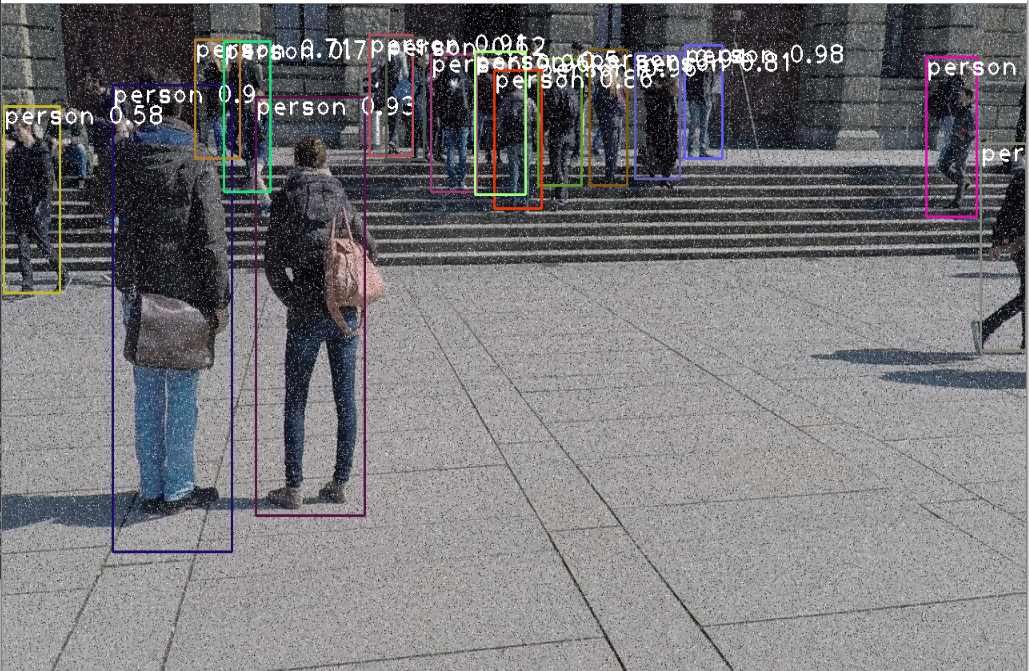
\includegraphics[width=65mm]{./images/appendix/imageAugment720pSandP.PNG}
	
	\vspace{2mm}
	\hspace{0.3mm}
	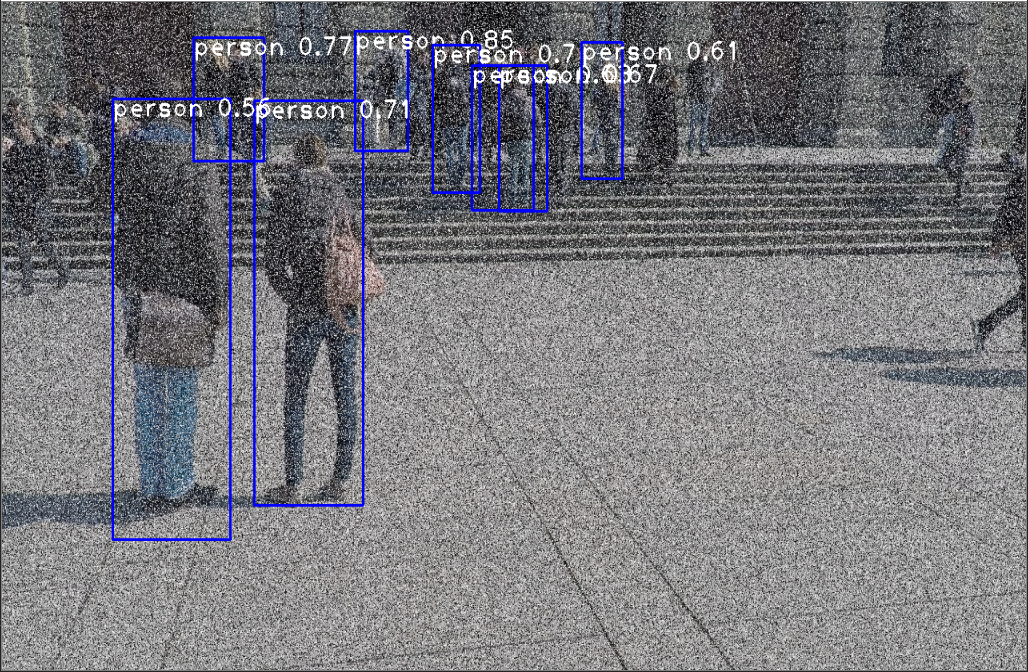
\includegraphics[width=65mm]{./images/appendix/imageAugment0.4SandP.PNG}
	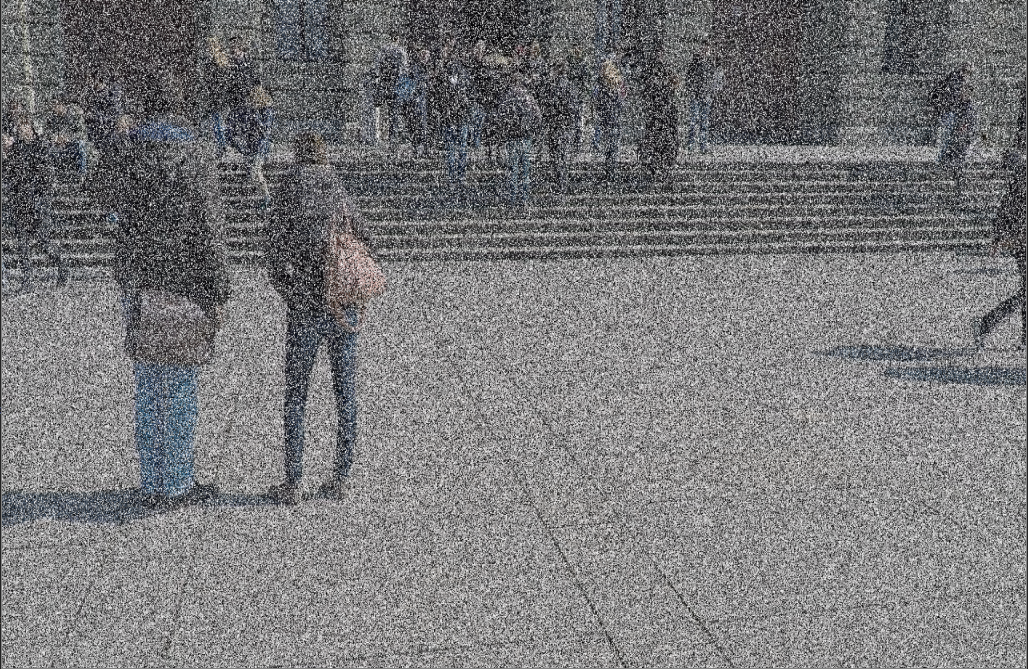
\includegraphics[width=65mm]{./images/appendix/imageAugment0.5SandP.PNG}
	\vspace{3mm}
	
	{\footnotesize Figure 5.2: 'Image 4' with artificial noise of 0,10,40,50 percent respectively}
\end{center}


\subsection{Conclusion for detecting objects}

The architecture worked well for all images that were tested but have limitations that can occur when an object blocks another. However, having a better camera angle will solve the issue and is recommended when using this system. Tuning the confidence and NMS effectiveness can be finicky and can differ depending on the camera quality used therefore testing different parameter values for the user's setup before using the system for surveillance is essential to avoid miscalculation.

\section{Using a video as an input}

A while loop is used to read each frame of the video in chronological order and is fed to the model. With the help of GPUs, the process of forwarding each frame to the network is sped up by roughly 4 times compared to using a CPU only. See appendix 4 for screenshots of 'video 3'

\vspace{2mm}

Beneficiaries are able to use their webcam/surveillance cameras as an input in real time with this implementation. The downside of running this program in real time with a camera of 30 frames per second is that it requires more GPU power compared to the results seen in the report. Currently the setup in this report computes the videos at approximately 10 frames per second. 

\section{Detecting social distancing by bounding box}

Using the bounding boxes that 'yolov3' architecture has identified, the system in theory should be able to mark the middle of every 'person' in the image/video. To calculate the middle of bounding box coordinates, the model provides the position of the left-upper corner of the bound box represented as (x,y) and also gives the height and width of the bounding box as h and w. Therefore:
\begin{equation*}
Middle Of Bounding Box Coordinates = (x+\frac{w}{2}, y+\frac{h}{2})
\end{equation*}


To calculate distance between every individual using the bounding boxes given, the system uses a 'for' loop of time complexity O($n^2$) to draw a line between every individual in the image/frame. The line can be measured using Pythagoras' theorem. Once calculated, the system filters lines that are below the social distancing threshold red, else the line is green. For the results produced, some green lines were filtered if they were larger than a certain threshold to give better clarity on the lines that showed 'not social distancing'. See appendix 4a for an example of all the lines in a single image.

\vspace{2mm}

For the first prototype of the system, the threshold of social distancing is measured by pixels. The first test uses 'image 4' with the threshold of 400 pixels being the social distancing length. This length was determined by measuring the two people who are next to each other with pixels (approximately 360 pixels apart) and slightly increasing the number. This also means that images from different cameras will need different threshold values due to the angle of the camera and the camera's focal length.

\vspace{2mm}

The results seen in figure 5.3 do correctly identify the two people as not social distancing between each other, but there are connections from the two people at the front to people at the back who are seen by the system as not social distancing when in reality they are far away. This is because the current system does not consider the field of view, therefore the image acts a top down view instead of looking a plane at an inclined angle.

\vspace{2mm}

This is not the only problem with the system as measuring distance at the middle of the bounding box with the y coordinate has inaccuracies as doing so assumes that every person in the photo is the same/average height which is not the case. A better solution for this is to view the ground as a planar surface, and use the bottom of the bounding boxes or person's feet as a mark/coordinate point when measuring distance. 

\begin{center}
	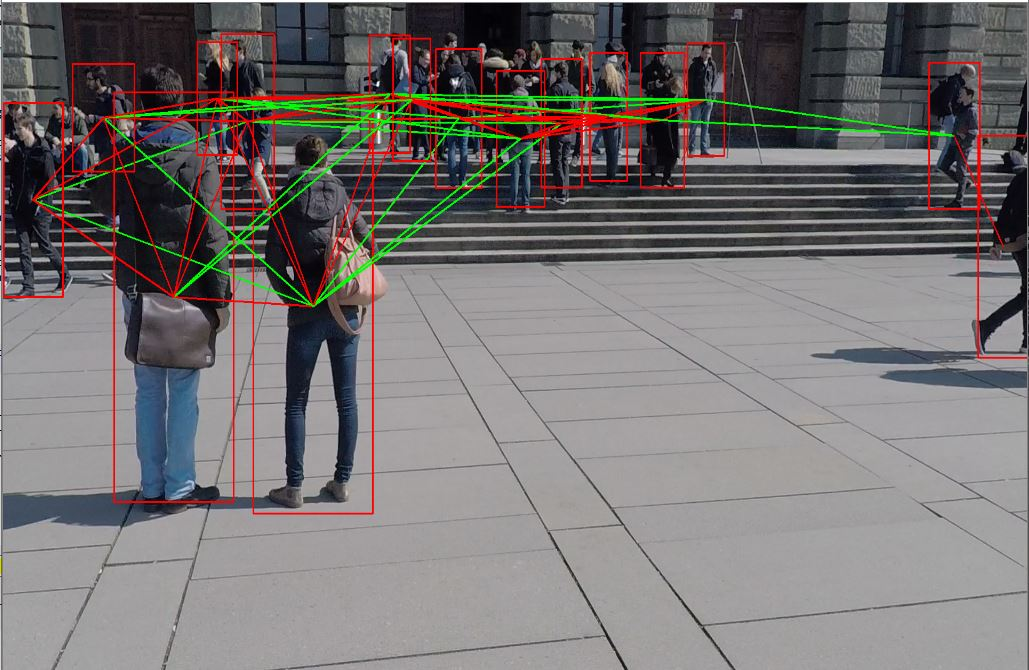
\includegraphics[width=65mm]{./images/appendix/test1.JPG}
	
	{\footnotesize Figure 5.3: 'Image 4' with first prototype social distancing detection}
\end{center}

\subsection*{Bounding box measurement improvement}

The first improvement to the system was to change the coordinates of where the line was being measured. Instead of using half of the bounding boxes' height added to the y coordinate, the system adds 99 percent of the height. 99 was specifically used because the bounding boxes generated by the model could sometimes overshoot the person's shoe, therefore using slightly less than the bounding box height would correct this. 

\vspace{2mm}

While the improvement to the system did not classify anyone people as 'social distancing', the connections coming out of the two people at the front and the people in the background  (Figure 5.4) are green, indicating that they are a safe enough distance. This improvement provides flexibility between the images/videos used in the dataset (See Appendix 4b for results on 'video 9'), as the implementation does not need to be tweaked when changing cameras. 

\begin{center}
	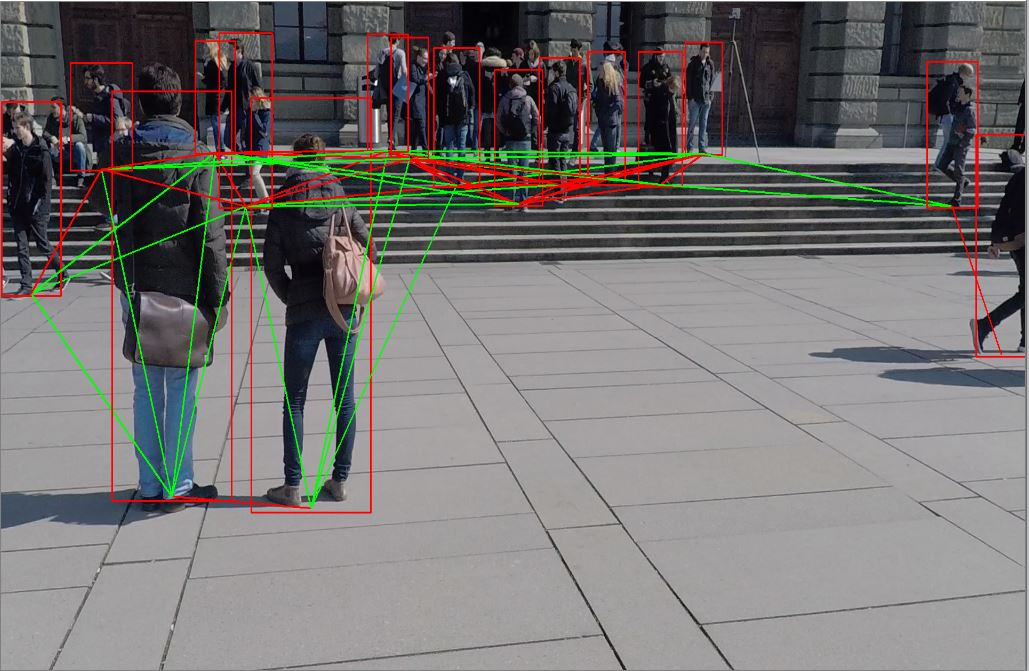
\includegraphics[width=80mm]{./images/appendix/BoundingBoxBottom.JPG}
	
	{\footnotesize Figure 5.4: 'Image 4' with measurement improvement.}
\end{center}

\subsection*{Solution to perspective distance}

Looking at the tiles of the floor in 'image 4', the tiles get smaller as they get further from the camera linearly. The rate at which they get smaller depends on several factors: the focal length of the camera and the distance from the camera. The equation to calculating the size of a person in the image respective to how far they are from the camera would be:

\begin{equation*}
Object Size In Image = Object Size * \frac{Focal Length}{Object Distance From Camera}
\end{equation*}

The implementation of this method will only rely on pixel distance between two bounding boxes, therefore we can not use the actual focal length of the camera and object distance from camera as parameters in the equation. Therefore a solution to this is to use the x and y coordinate of the bounding boxes to determine how far the person is from the camera, where the smaller the y, the further the object is from the camera. (the coordinate (0,0) starts at the top left-hand corner of the image.)

\vspace{2mm}

The first solution was to multiply every y coordinate by 2 while keeping the threshold the same (400 pixel distance). This in theory is the focal length parameter as an estimate and also could be seen as a stretch in the x axis. People who are on the same y coordinate are in the same perspective distance, therefore multiplying the y coordinate will have very little effect on people who have the same y value when calculating Pythagoras where as people who are on different y coordinates with be impacted greatly. 

\vspace{2mm}

The results (Figure 5.5) show a large improvement to the previous version, being able to classify 3 different people as 'social distancing' unlike figure 5.4. The implementation still classified the two people at the front as not 'social distancing' which is a success.

\begin{center}
	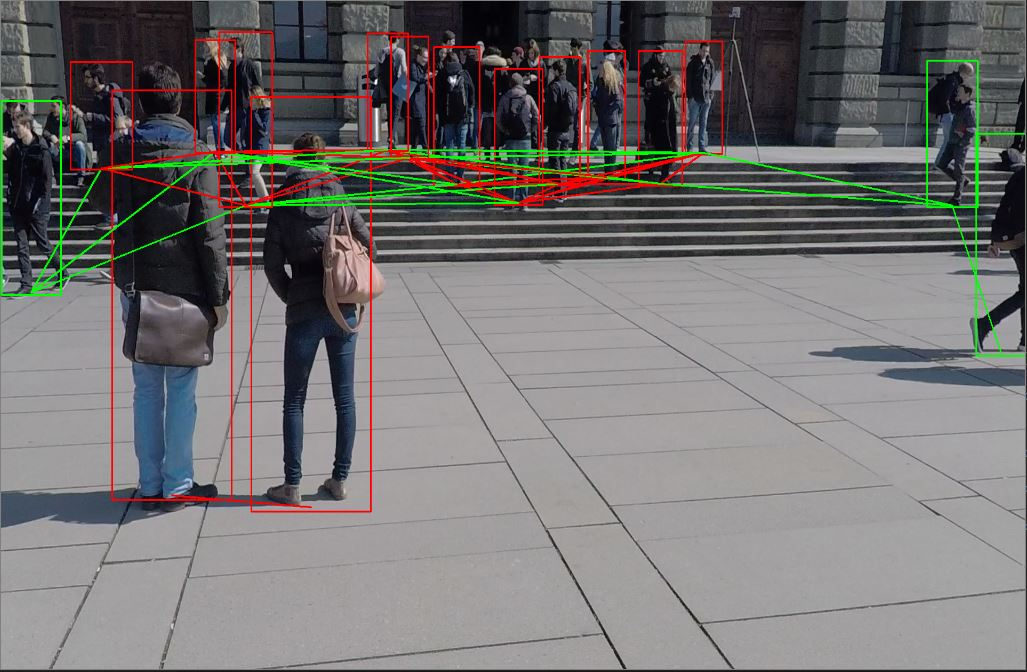
\includegraphics[width=80mm]{./images/appendix/PerspectiveSolution1.JPG}
	
	{\footnotesize Figure 5.5: 'Image 4' with measurement improvement.}
\end{center}

While this is an improvement, the perspective is only 'solved' in the y axis. As things are further away from the camera or the y coordinate becomes smaller, each pixel represents a larger area in the real world. Therefore the system would need to scale the threshold depending on the value of the y coordinate. The equation used to calculate the new threshold with respect to the y coordinate is:

\begin{equation*}
UpdatedThreshold = OriginalThreshold - \frac{OriginalY*Scalar}{MeanCoordinateBetweenObjects}
\end{equation*}

The 'OriginalY' variable is based of the y coordinates of where the 'OrginalThreshold' was measured (This can be referred from the first prototype of the implementation.). In 'Image 4' case, the 'OriginalY' is the mean y coordinate between the two people at the front (value 800). 

\vspace{2mm}

Figure 5.6 showcases the before and after of the 'threshold scalar' implementation using the different 'scalar' value at 20, 40, 50 respectively. The turquoise lines indicate not 'social distancing' between people. While  the implementation does not classify anyone new as being 'social distancing' with the 'scalar' value being 20, some lines are removed between the two cluster of people in the background. The reductions of lines seen between the before and after indicate that the equation discussed previously is working as intended.

\vspace{2mm}

As the scalar increases, less and less connections appear in the final output of the image and more people are highlighted in green which means that they are 'social distancing'. With the 'scalar' variable being 50, only adjacent people are connect with lines. The method is very effective at dealing with perspective distance as the two people at the front are still classified as not 'social distancing'.

\begin{center}
	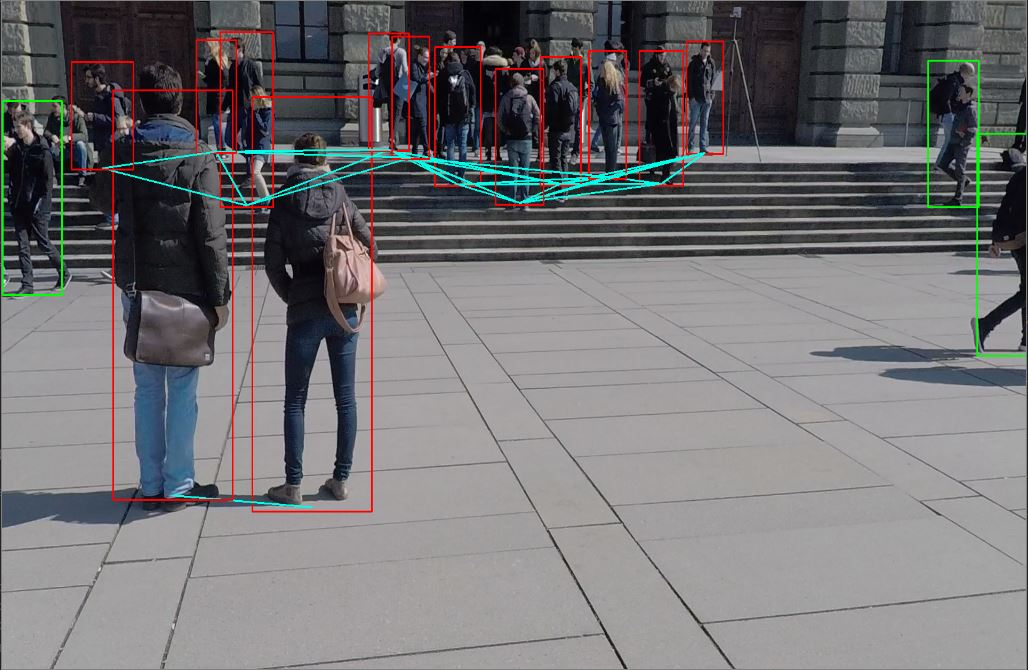
\includegraphics[width=65mm]{./images/appendix/BeforeThresholdScale.JPG}
	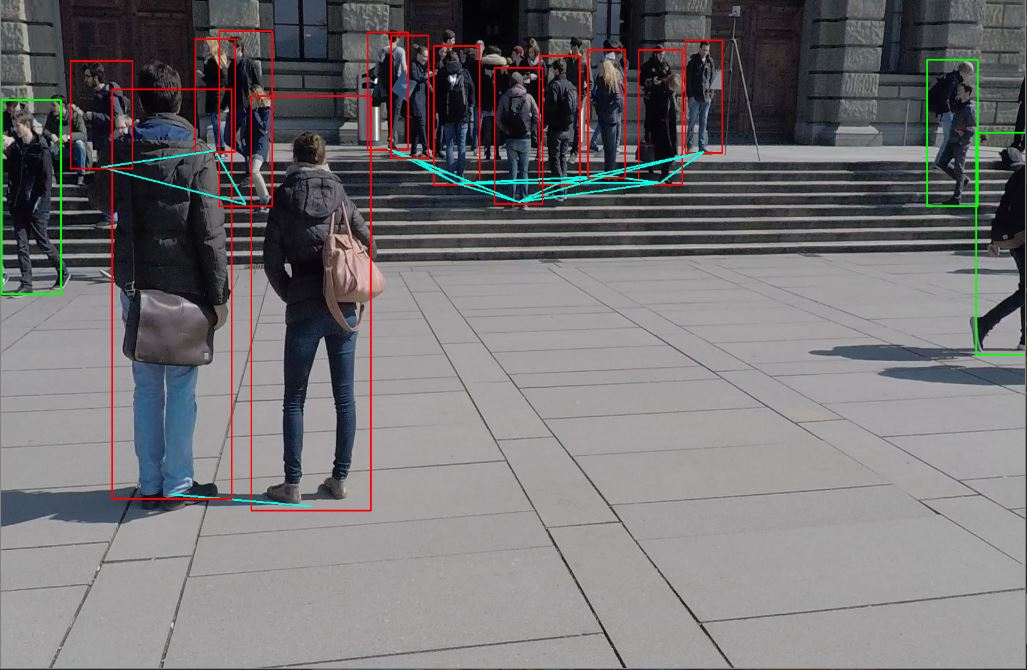
\includegraphics[width=65mm]{./images/appendix/AfterThresholdScale.JPG}
	
	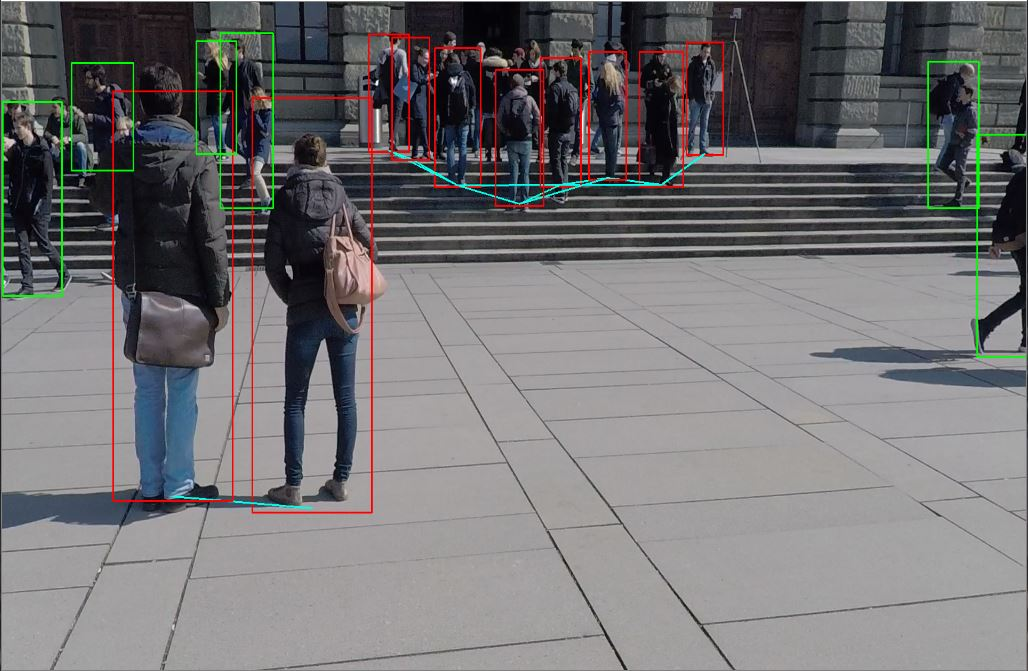
\includegraphics[width=65mm]{./images/appendix/AfterThresholdScale40.JPG}
	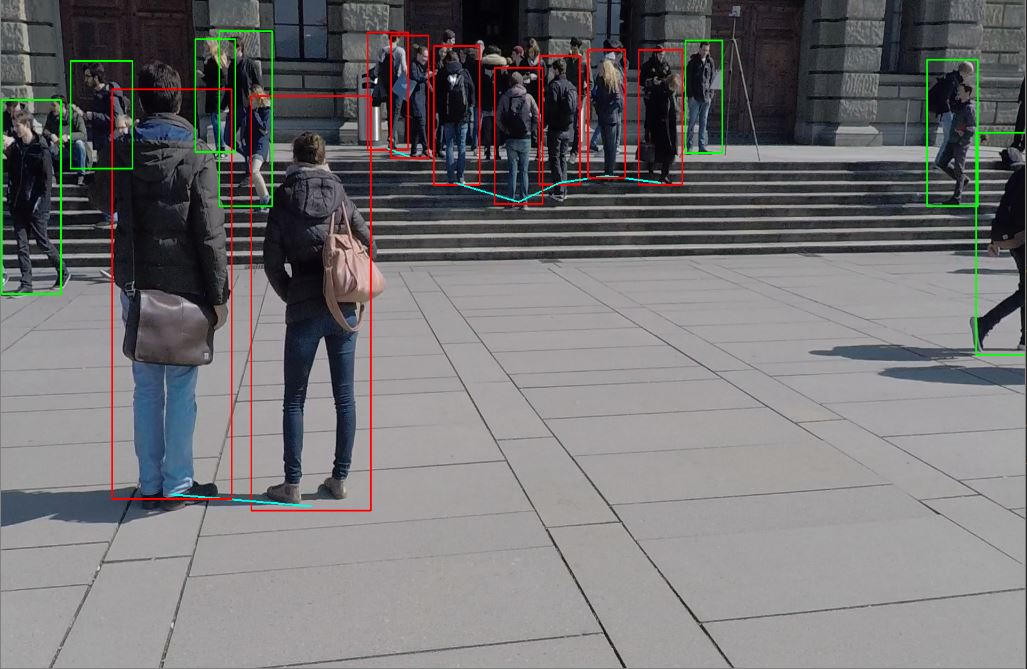
\includegraphics[width=65mm]{./images/appendix/AfterThresholdScale50.JPG}
	
	{\footnotesize Figure 5.6: 'Image 4' before and after scalar adjustments (Non,20,40,50 respectively).}
\end{center}

\subsection{Conclusion of detecting SD by bounding box}

The final output of the method worked as intended. The combination of the two equations discussed could be seen as rotating a line in a 3d space to be fixed on a plane or two separate transformation (stretch) to the image to account for the incline angle the camera has to the floor of the image.

\begin{center}
	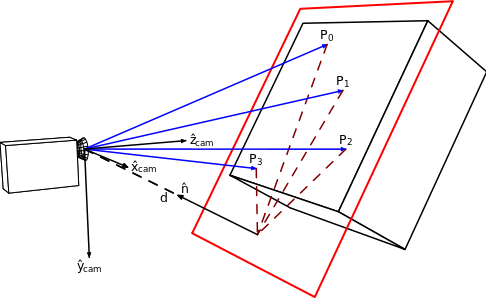
\includegraphics[width=65mm]{./images/appendix/qwe.JPG}
\end{center}

The problems that this implementation has are that the measurements are pixel values and not real word value, therefore we cannot know the exact distance between each person. Solutions such as giving a single pixel a defined real world measurement is plausible by using the average measurements of an object for scale with respective to a pixel, but the value will vary depending on the different focal lengths each camera has.

\vspace{2mm}

Another problem with this method is that the beneficiaries will have to tune the variables in the equation if they choose to use this for detecting social distancing. It is very likely that their setup is different and getting reasonable numbers for the variables will takes a lot of trial and error. 
In conclusion, this solution is only an estimate to calculating social distancing and is nowhere near perfect. 

\section{Detecting social distancing by matrix transformation}

The previous method uses the floor in the images/videos as a planar surface for better precision when calculating the final output. This method takes the same ideas and uses a matrix transformation to augment the image into a top down view. This is done by selecting 4 points in the image where each point is pointing towards the floor (Most likely the points connect to a irregular quadrilateral). The system is able to utilise a function from OpenCV called 'getPerspectiveTransform' which is able to calculate a matrix that transforms the 4  connected points to another irregular quadrilateral or rectangle. The relationship between the images produce is called homography (OpenCV: Basic concepts of the homography explained with code, 2021) as they both represent the same planar surface in the real world.

Once the matrix is acquired, OpenCV has another function that  


\chapter*{Appendix}

\section*{Appendix 1: YOLO flowchart}

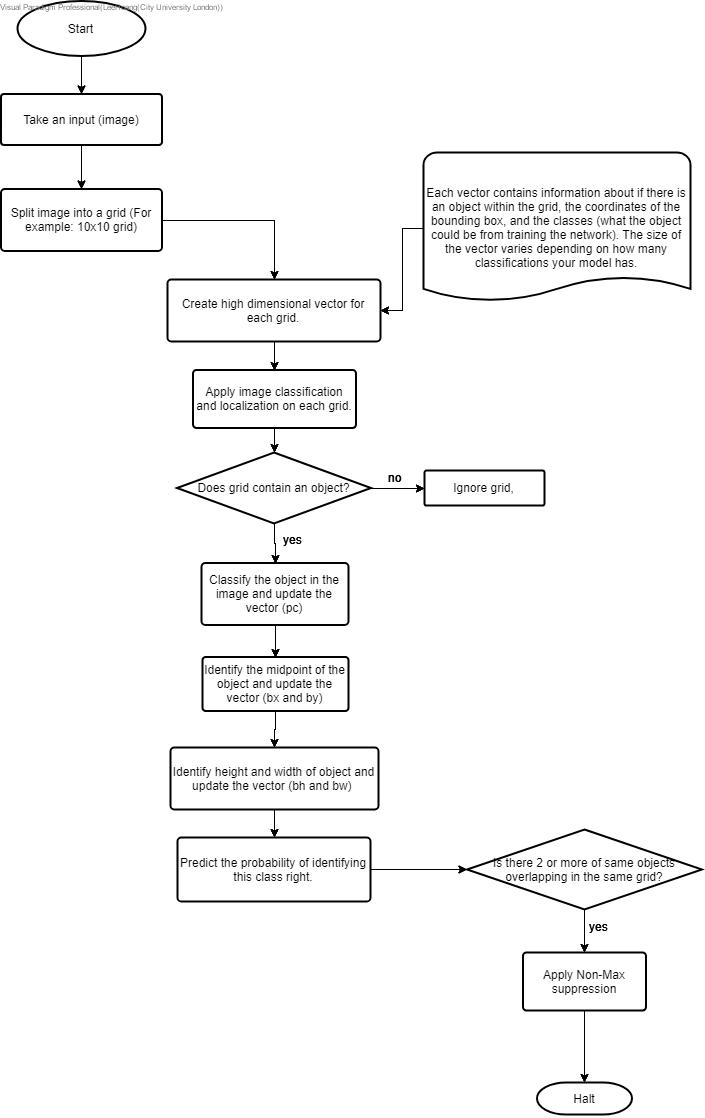
\includegraphics[width=110mm]{./images/YOLO.jpg}

\section*{Appendix 2: System class diagram}

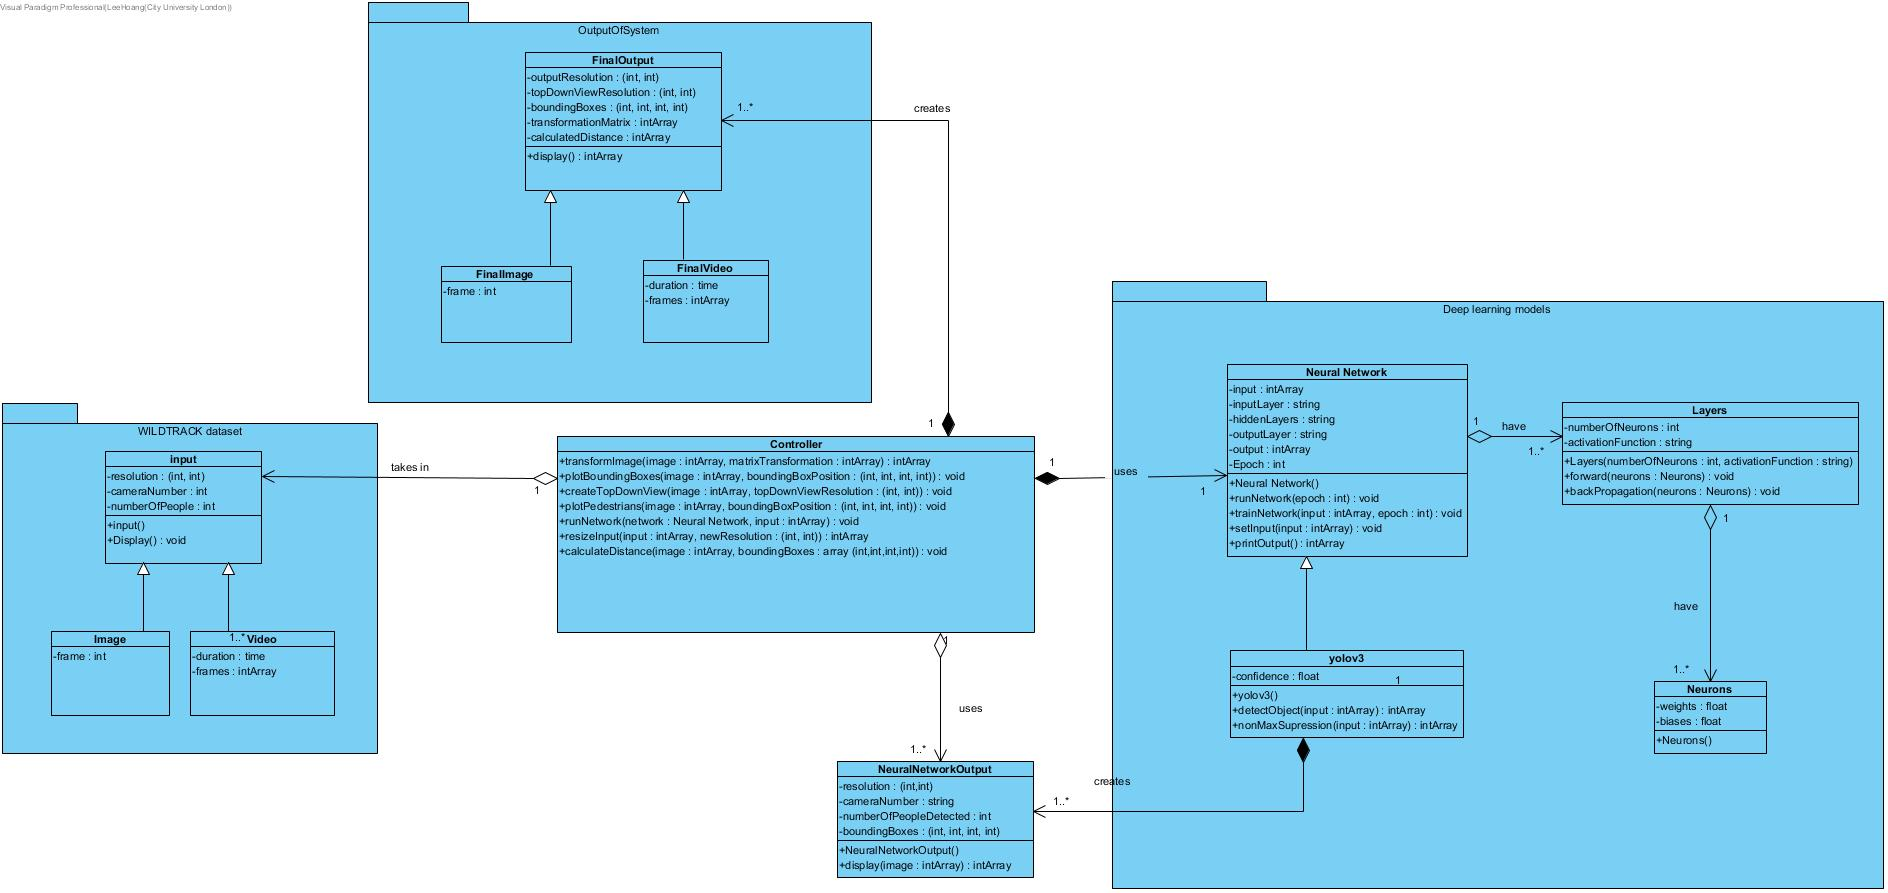
\includegraphics[angle = 90,width=100mm]{./images/SD Class diagram.jpg}

\section*{Appendix 3: 5.1 outputs}

a)

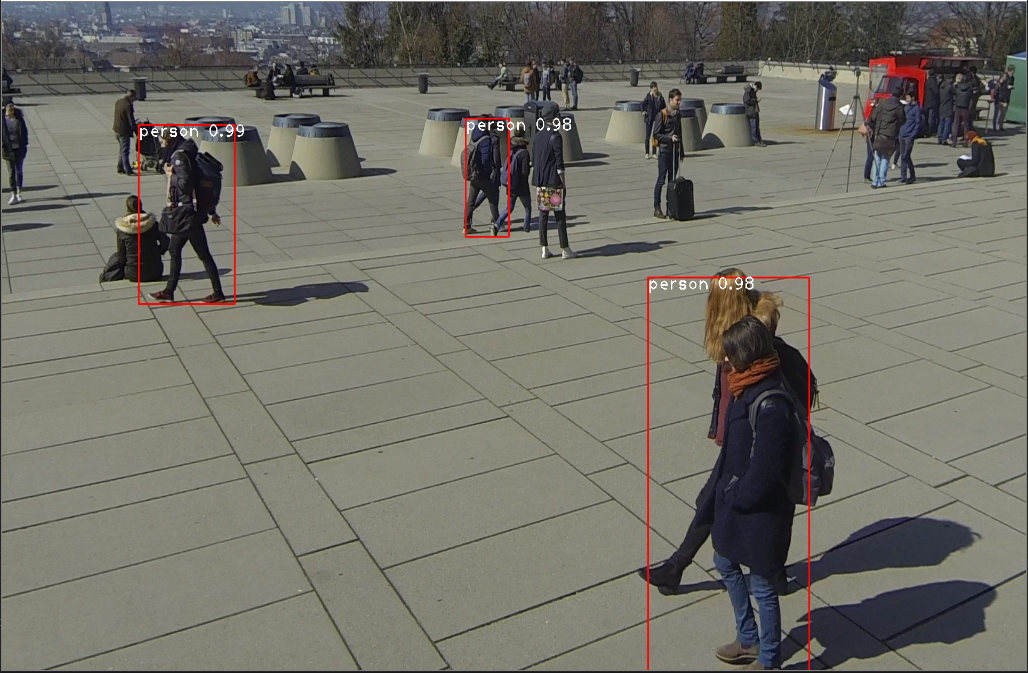
\includegraphics[width=120mm]{./images/appendix/image298confidence.PNG}

b)

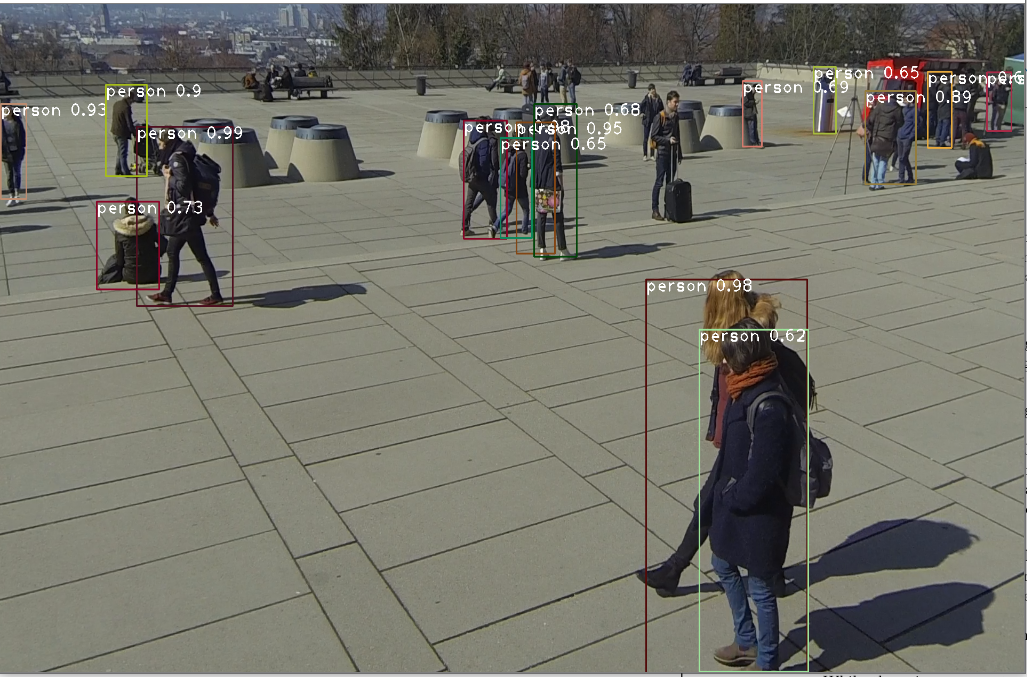
\includegraphics[width=120mm]{./images/appendix/NMS0.6.PNG}

c)

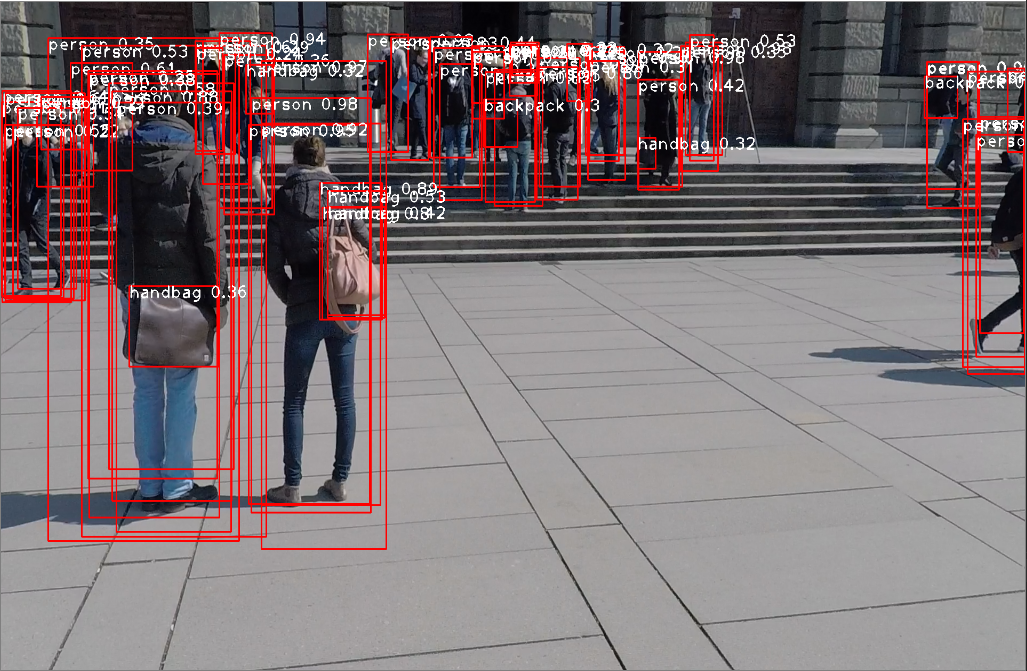
\includegraphics[width=70mm]{./images/appendix/NoConfidenceNoAug.PNG}
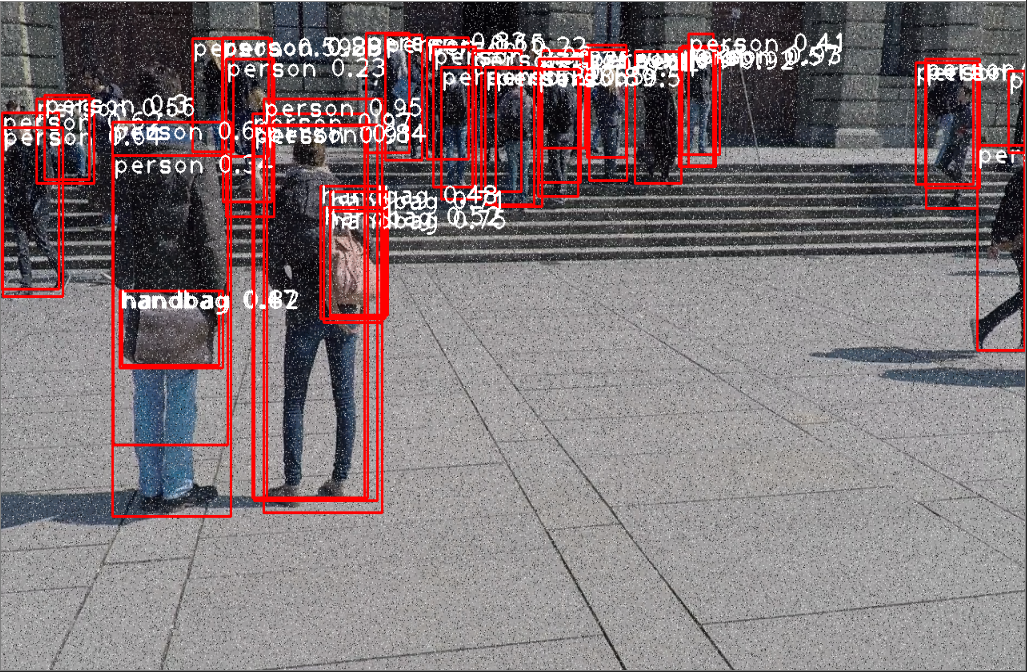
\includegraphics[width=70mm]{./images/appendix/NoConfidenceAug10.PNG}

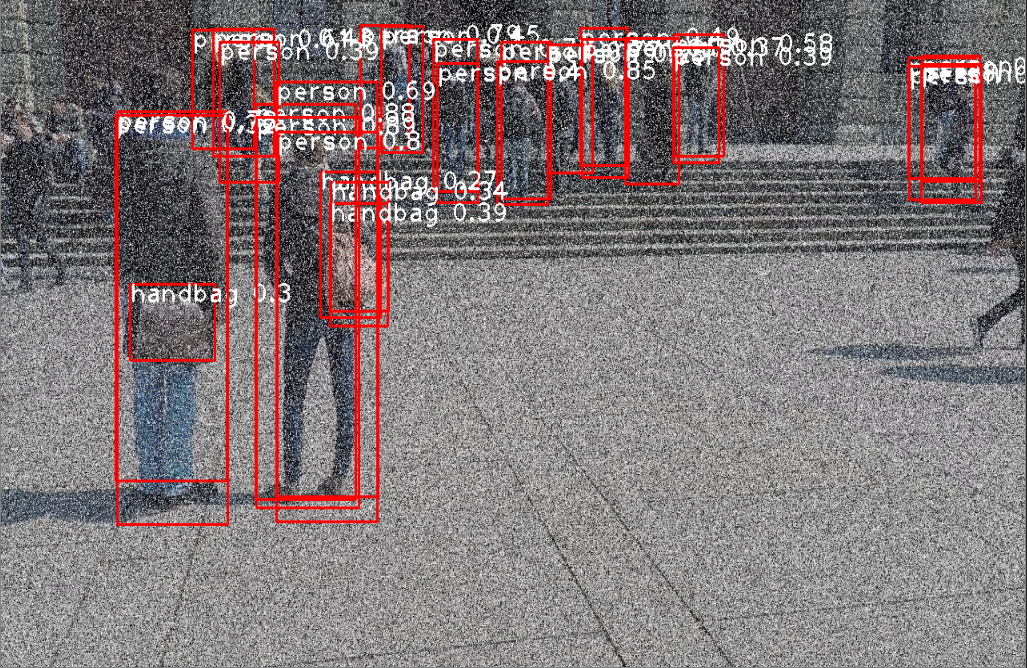
\includegraphics[width=70mm]{./images/appendix/NoConfidenceAug40.PNG}
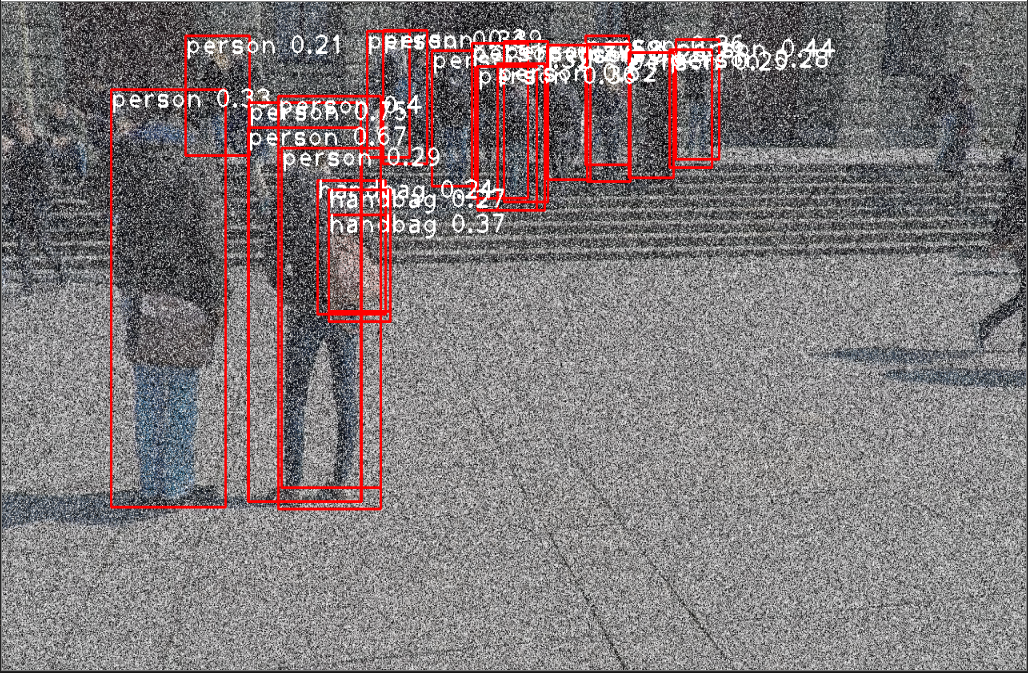
\includegraphics[width=70mm]{./images/appendix/NoConfidenceAug50.PNG}

\section*{Appendix 4: 5.2 outputs}

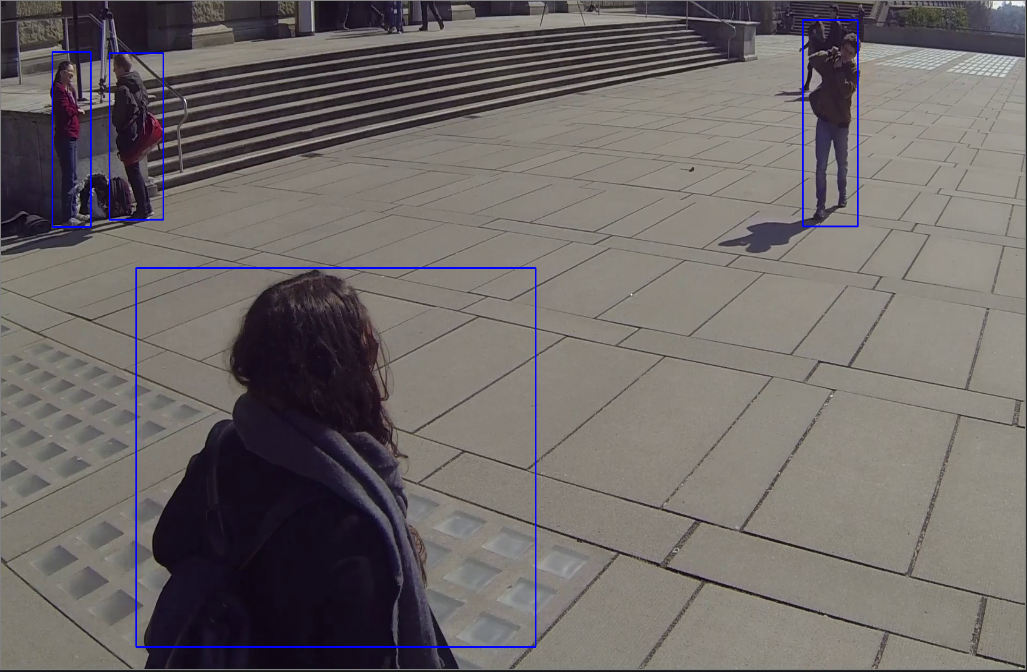
\includegraphics[width=70mm]{./images/appendix/Video3output1.PNG}
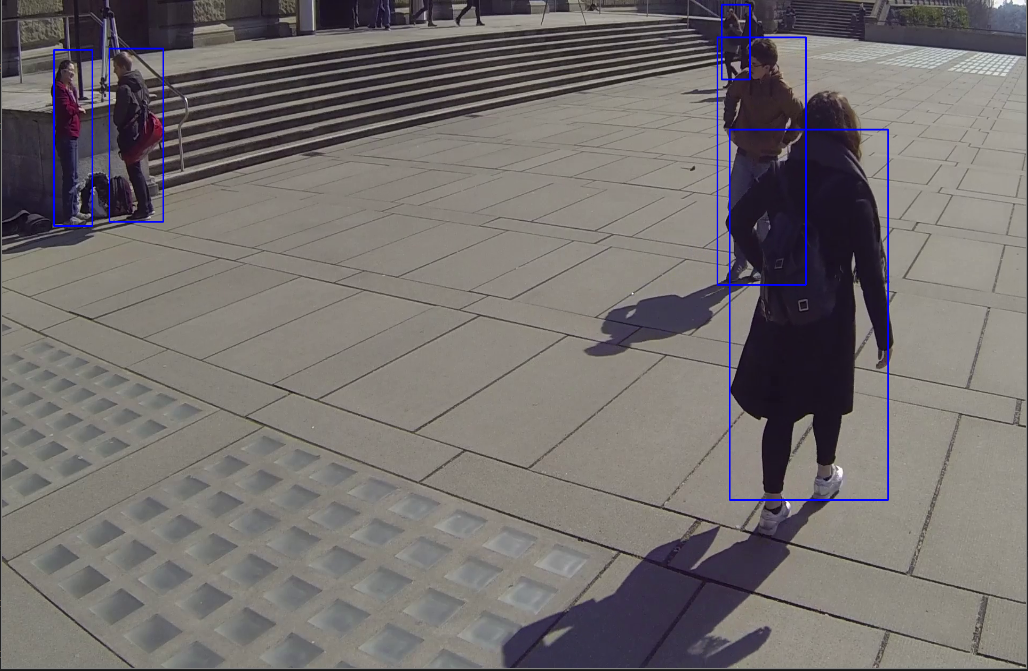
\includegraphics[width=70mm]{./images/appendix/Video3output2.PNG}


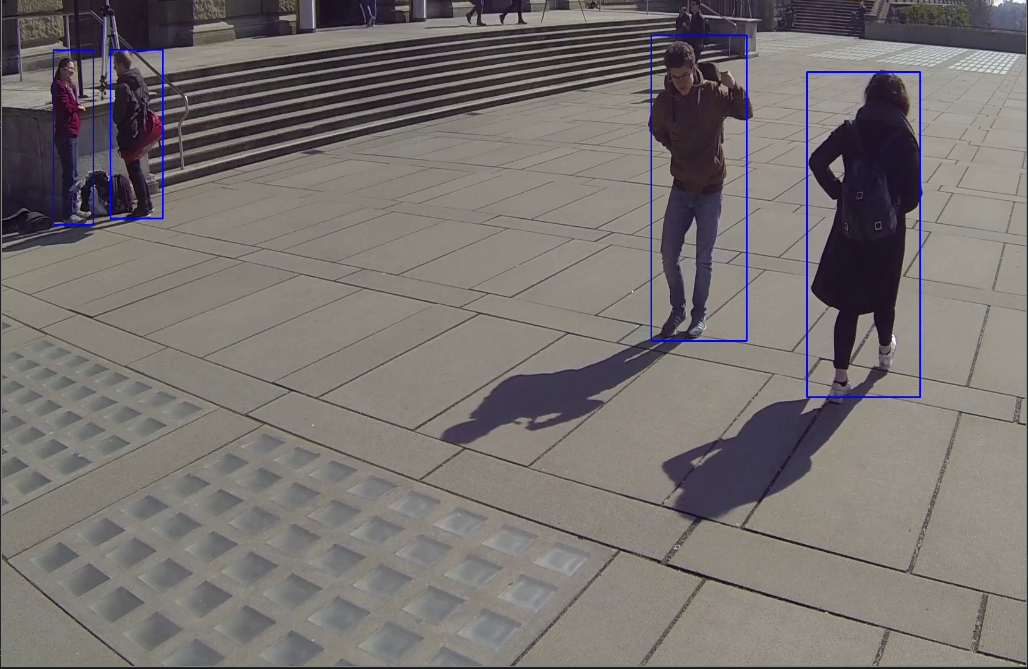
\includegraphics[width=70mm]{./images/appendix/Video3output3.PNG}
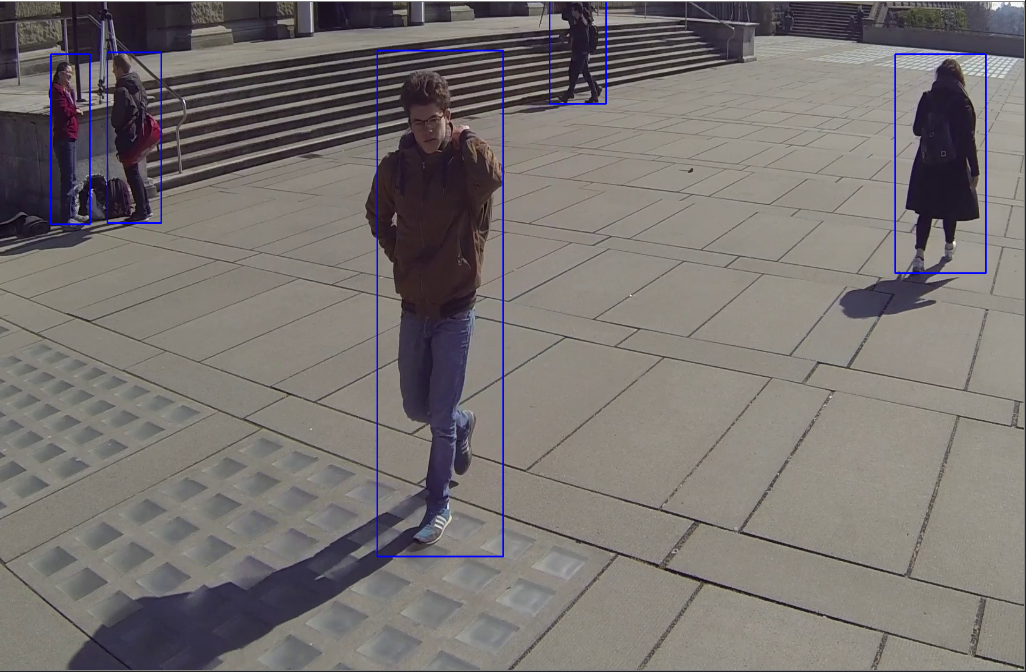
\includegraphics[width=70mm]{./images/appendix/Video3output4.PNG}

\section*{Appendix 4: 5.3 outputs}
a)


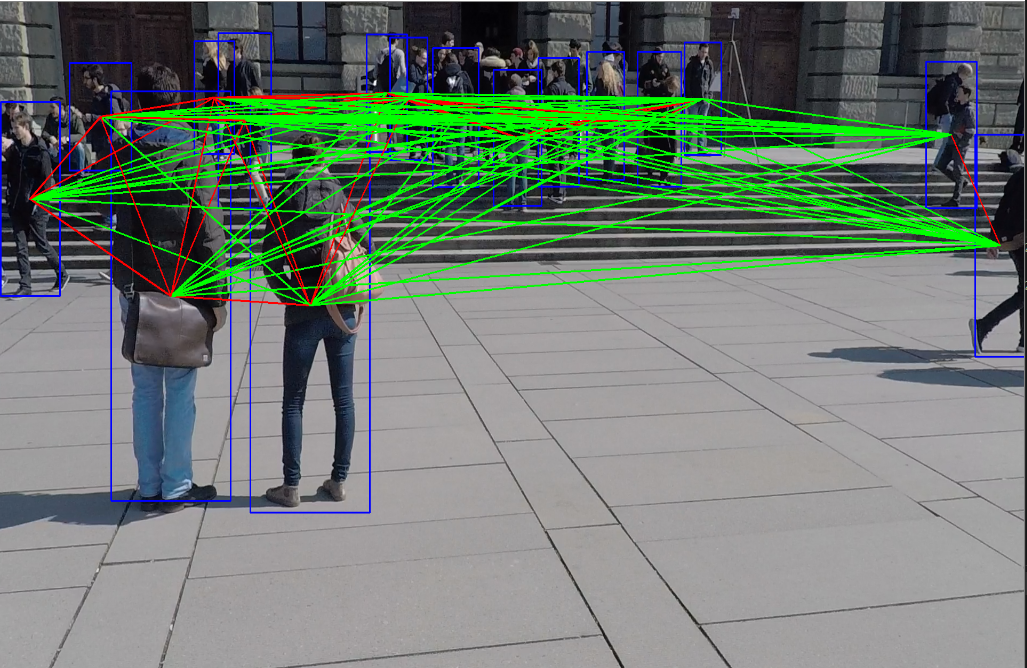
\includegraphics[width=120mm]{./images/appendix/SDNoFilterByPixel.PNG}

b)


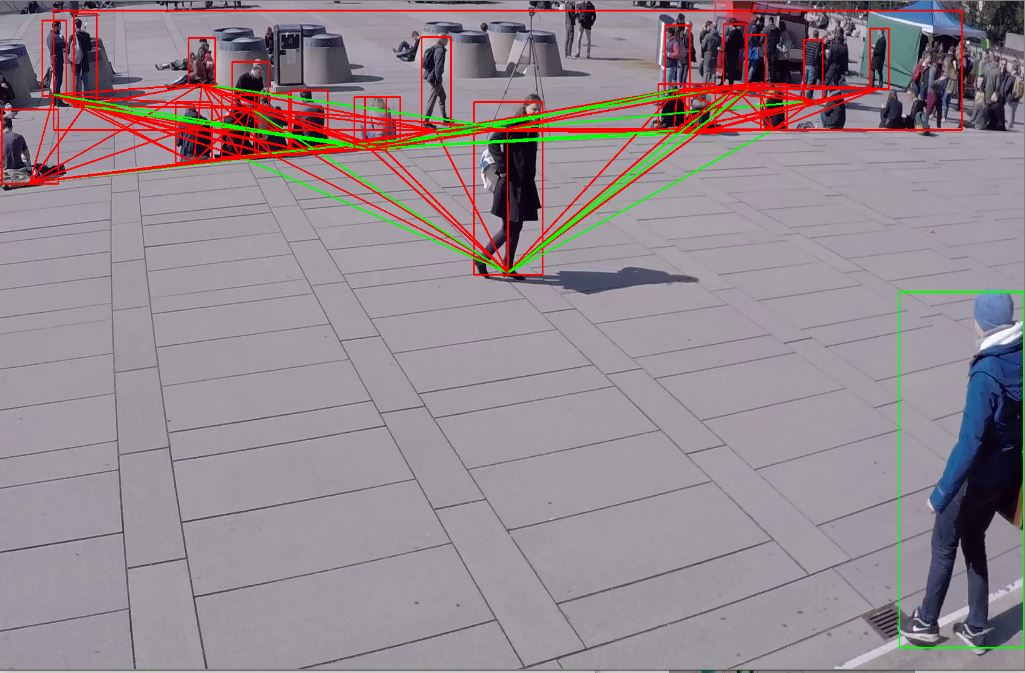
\includegraphics[width=70mm]{./images/appendix/Cam7Clip1BoundingBoxTest1.JPG}
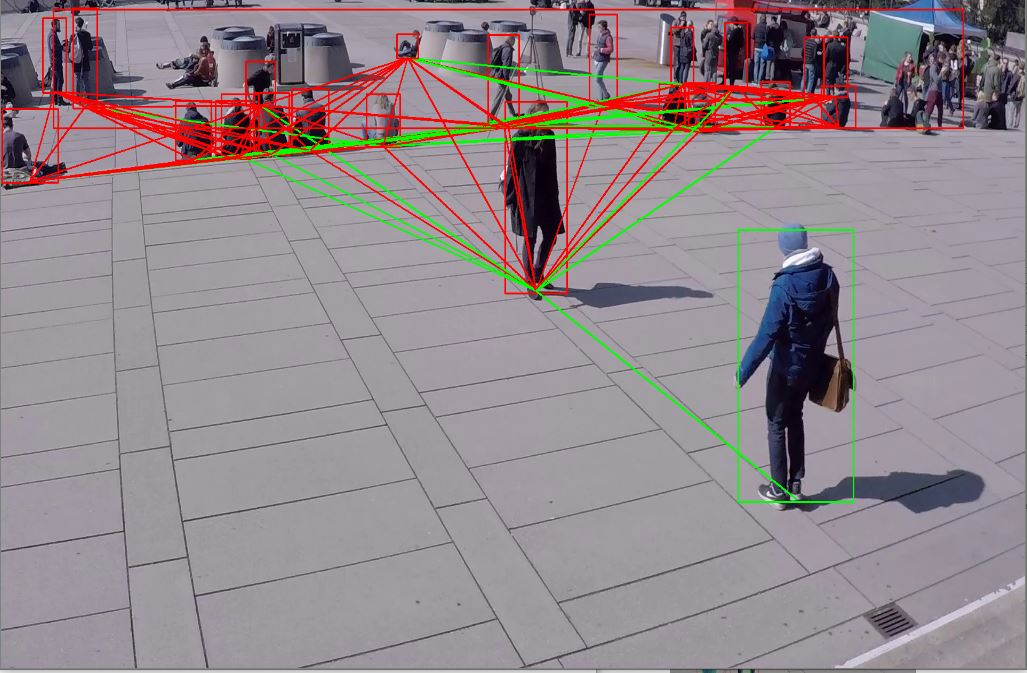
\includegraphics[width=70mm]{./images/appendix/Cam7Clip1BoundingBoxTest2.JPG}

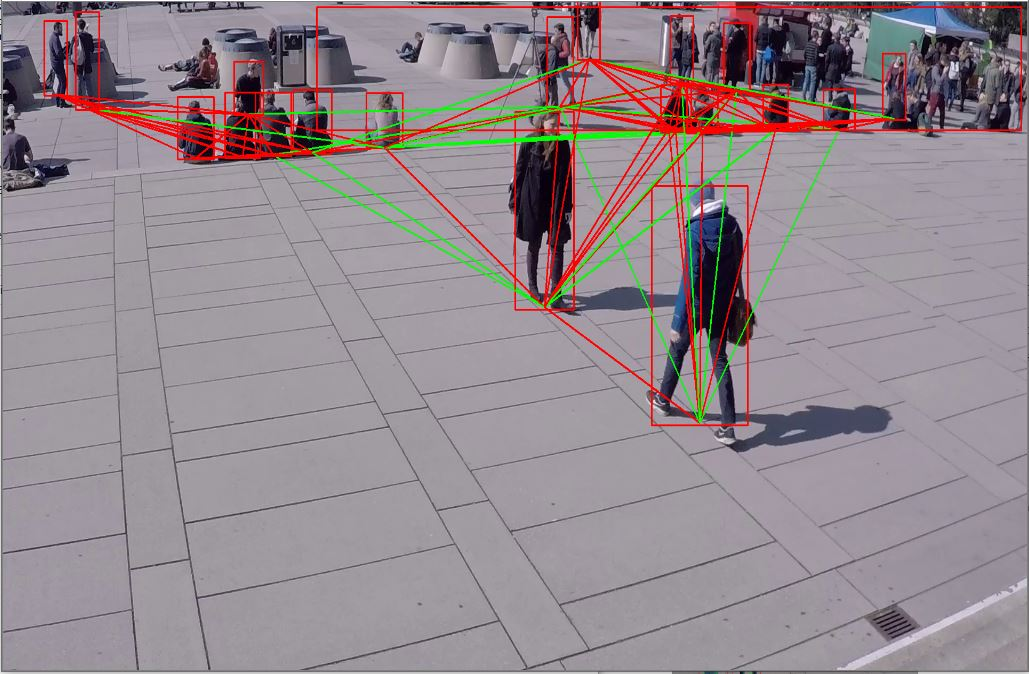
\includegraphics[width=70mm]{./images/appendix/Cam7Clip1BoundingBoxTest3.JPG}
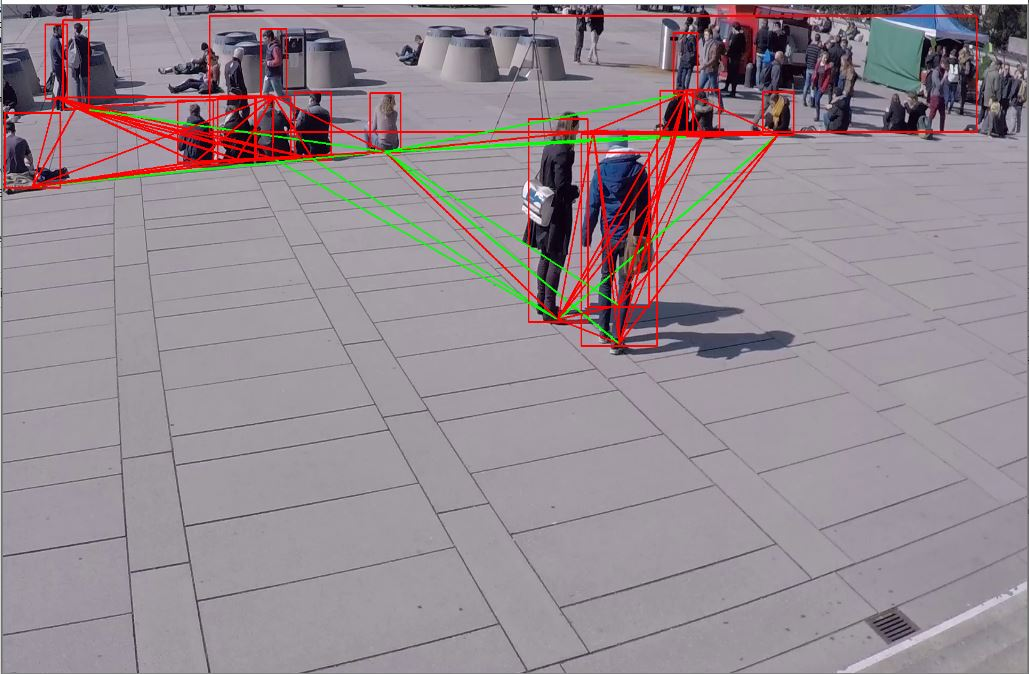
\includegraphics[width=70mm]{./images/appendix/Cam7Clip1BoundingBoxTest5.JPG}

\end{document}

